\section{Experiments}
\texttt{What you have found: The results should be  the larger part of the report.}

\subsection{Monk's results}
\begin{table}[H]
\begin{tabular}{|c|c|c|c|c|c|c|}
\hline
\textbf{Task} &	\textbf{\#Units} &\textbf{ eta} & \textbf{lambda} &\textbf{momentum} & {\textbf{MSE(TR/TS)}} &\textbf{Accuracy(TR/TS)} \\ \hline
MONK 1        &    3 & 0.9 & 0 & 0.7  &   6.3e-4/1e-3 &   100\%/100\%  \\ \hline
MONK 2        &    4 & 0.8 & 0 & 0.7  &   1e-3/1.3e-3 &   100\%/100\% \\ \hline               
MONK 3        &    5 & 0.4 &1e-3 &0.2&     4.1e-2/2.5e-2&    93.44\%/97.22\%  \\ \hline
MONK 3 (no reg)&   5 & 0.8 &   0 &  0.7 &   1.8e-2/2.6e-2 & 95.90\%/93.51\%		\\ \hline              
\end{tabular}
\end{table}
\subsubsection{Monk 1}

\begin{figure}[H]
    \centering
    \begin{minipage}[t]{0.5\linewidth}
        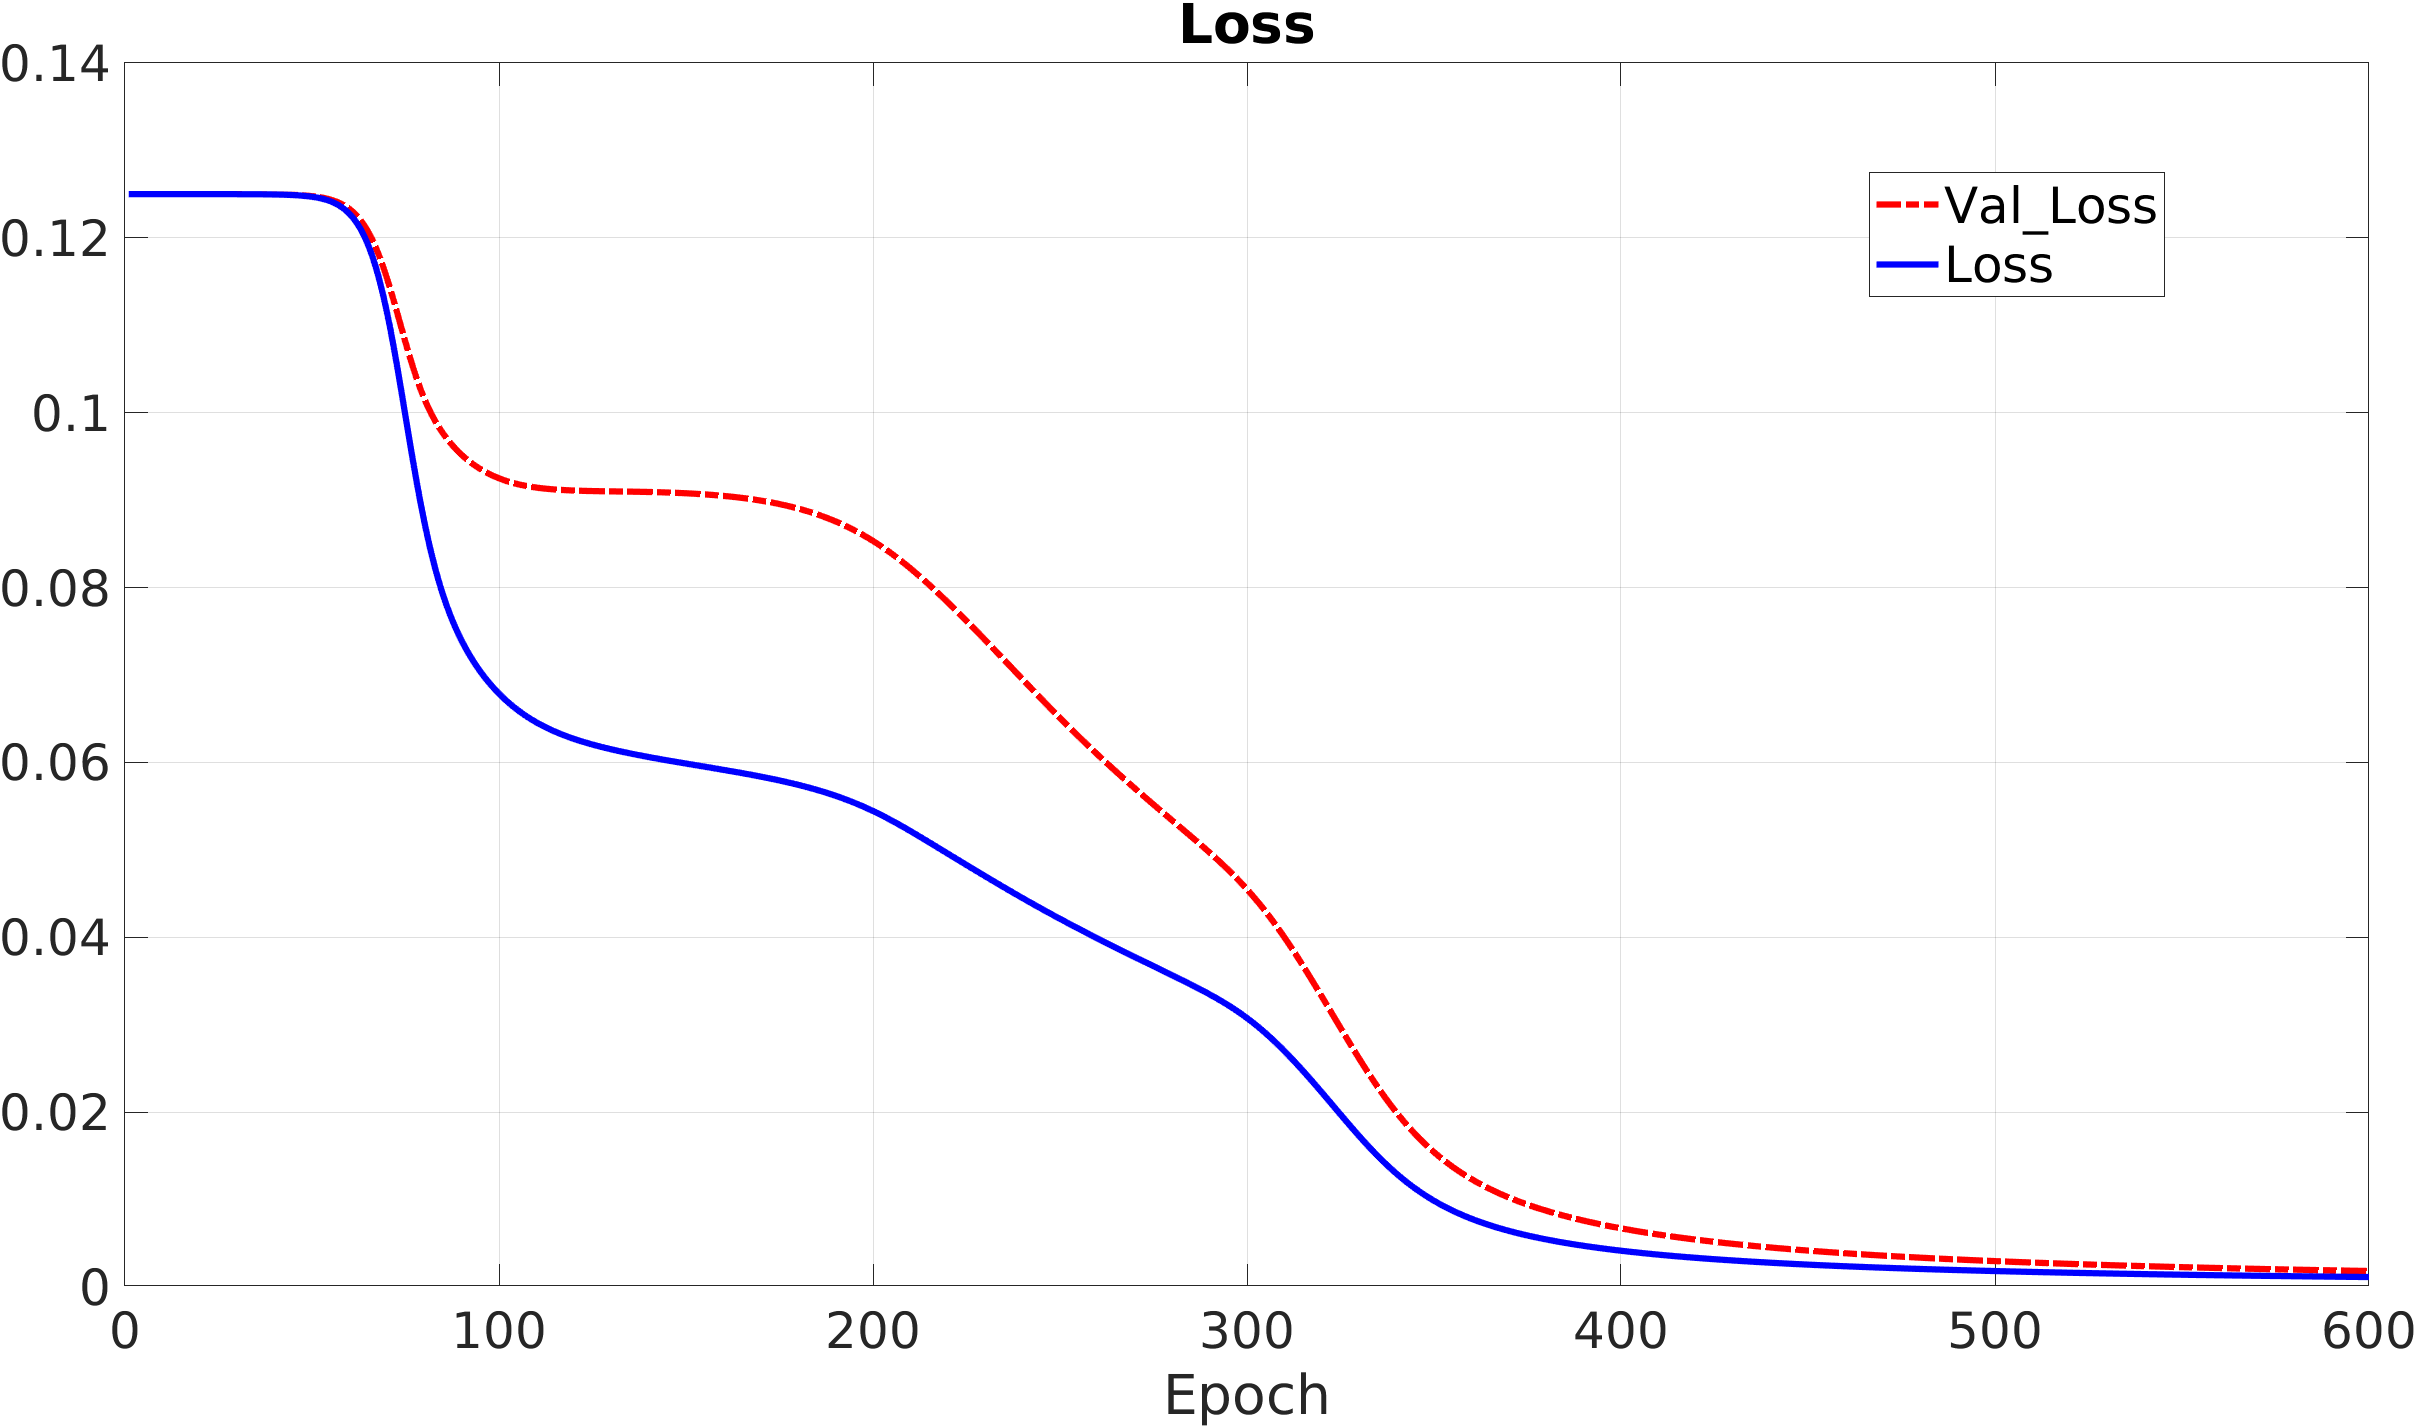
\includegraphics[width=\linewidth]{img/Monk1_loss.png}
        %\subcaption{MSE}
    \end{minipage}%
    \begin{minipage}[t]{0.5\linewidth}
        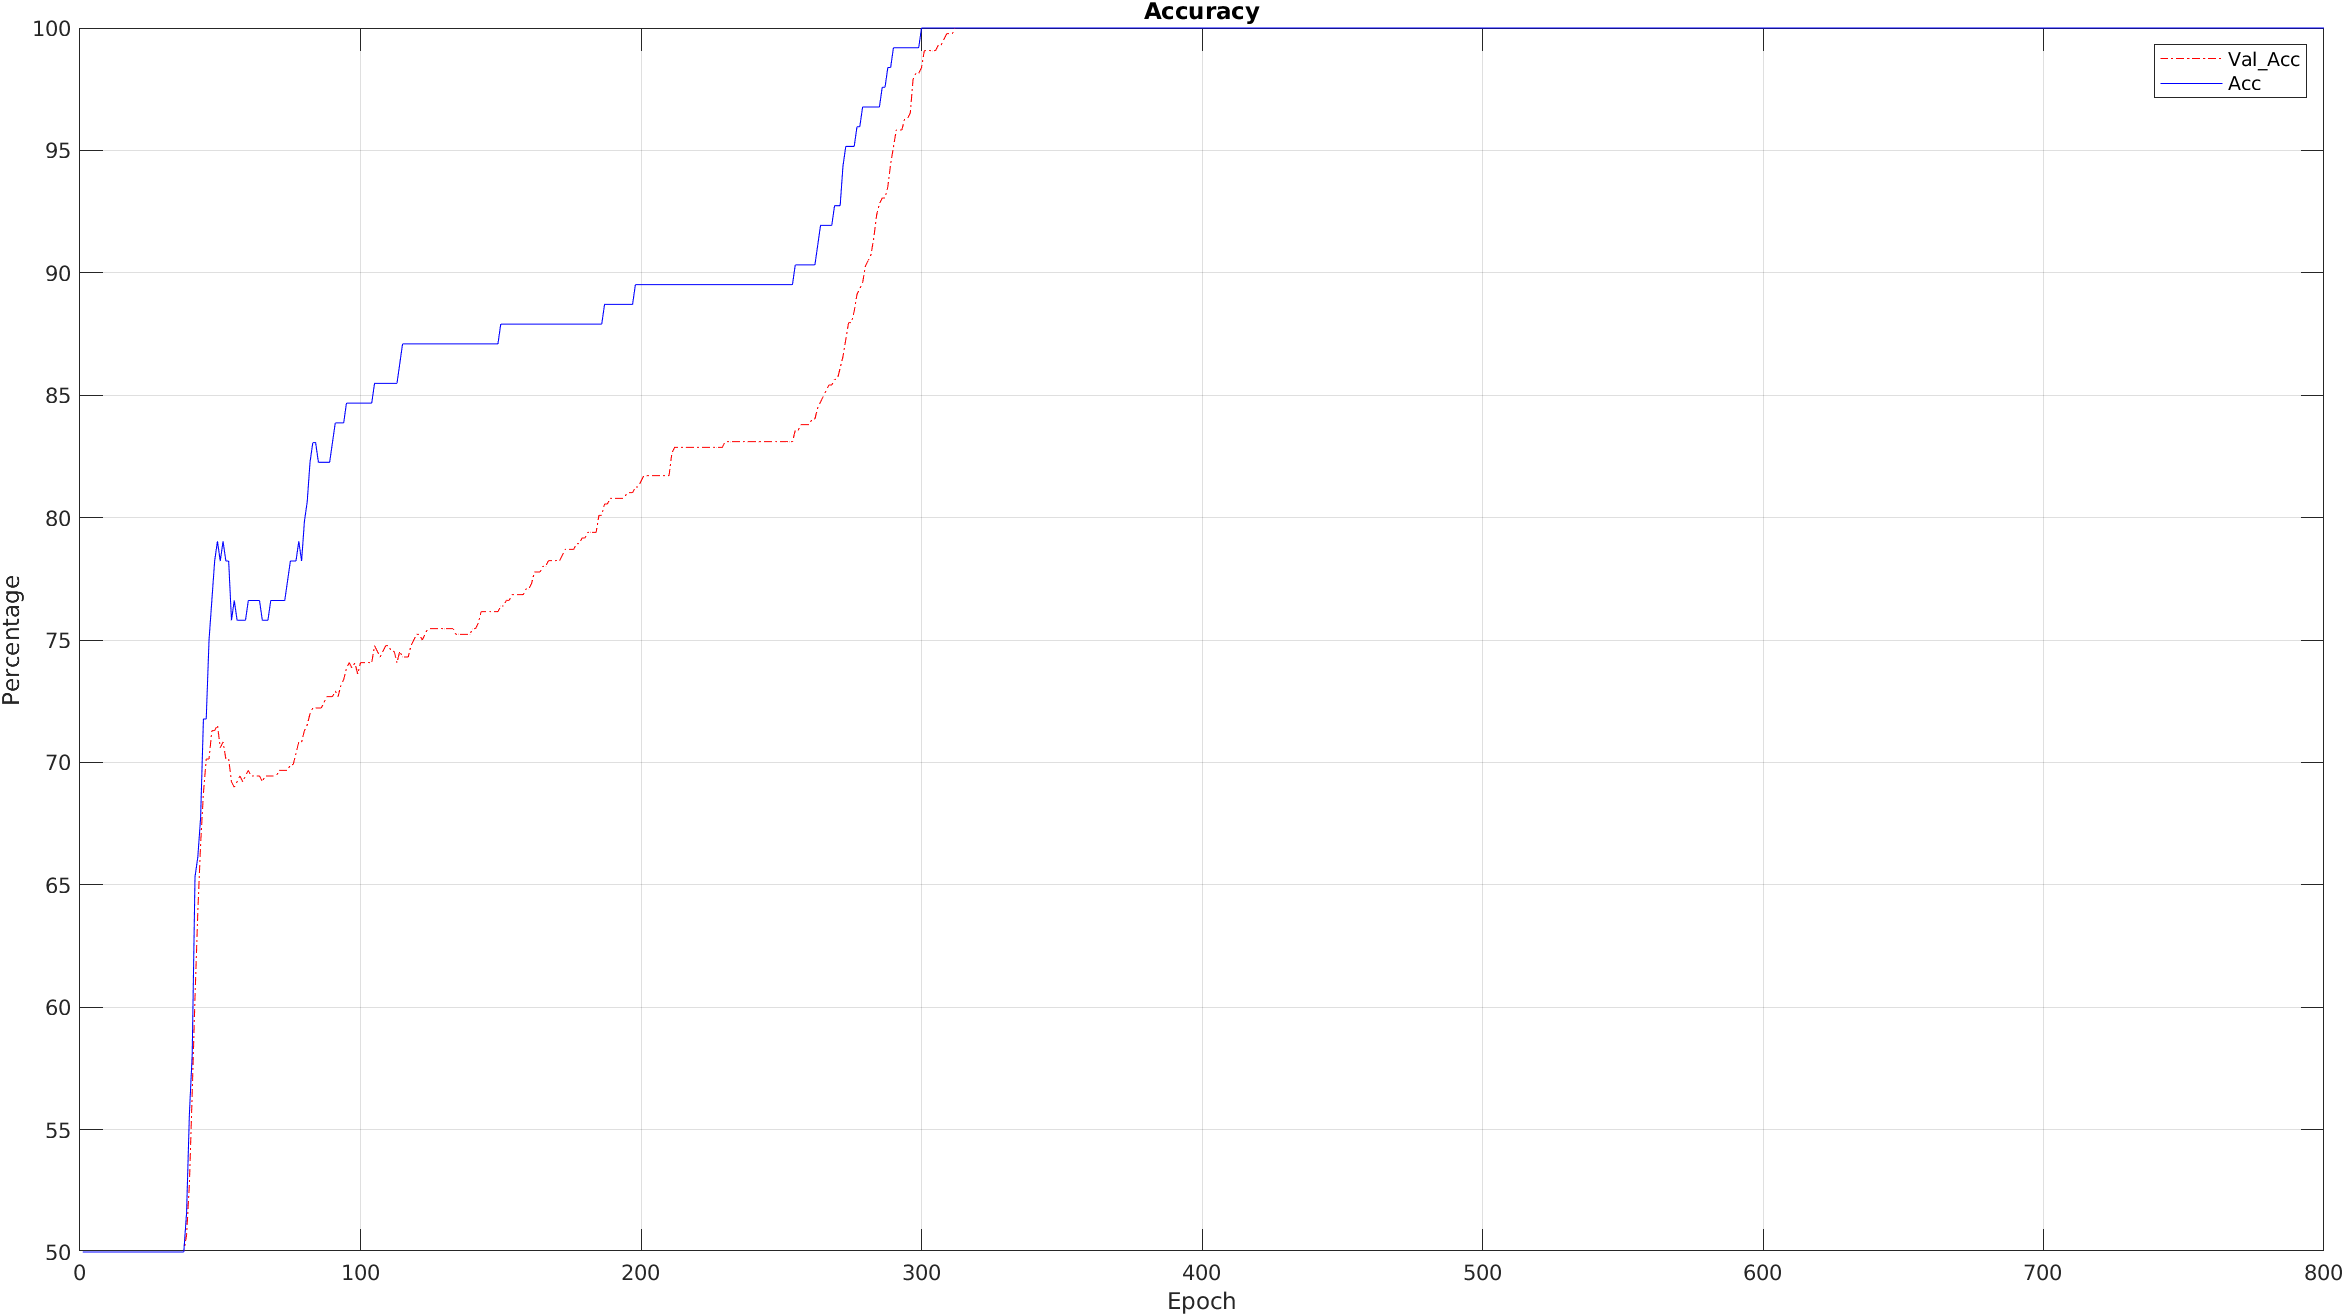
\includegraphics[width=\linewidth]{img/Monk1_accuracy.png}
        %\subcaption{Accuracy}
    \end{minipage}
    \caption{MSE and accuracy for MONK’s 1.}
\end{figure}

\subsubsection{Monk 2}
\begin{figure}[H]
    \centering
    \begin{minipage}[t]{0.5\linewidth}
        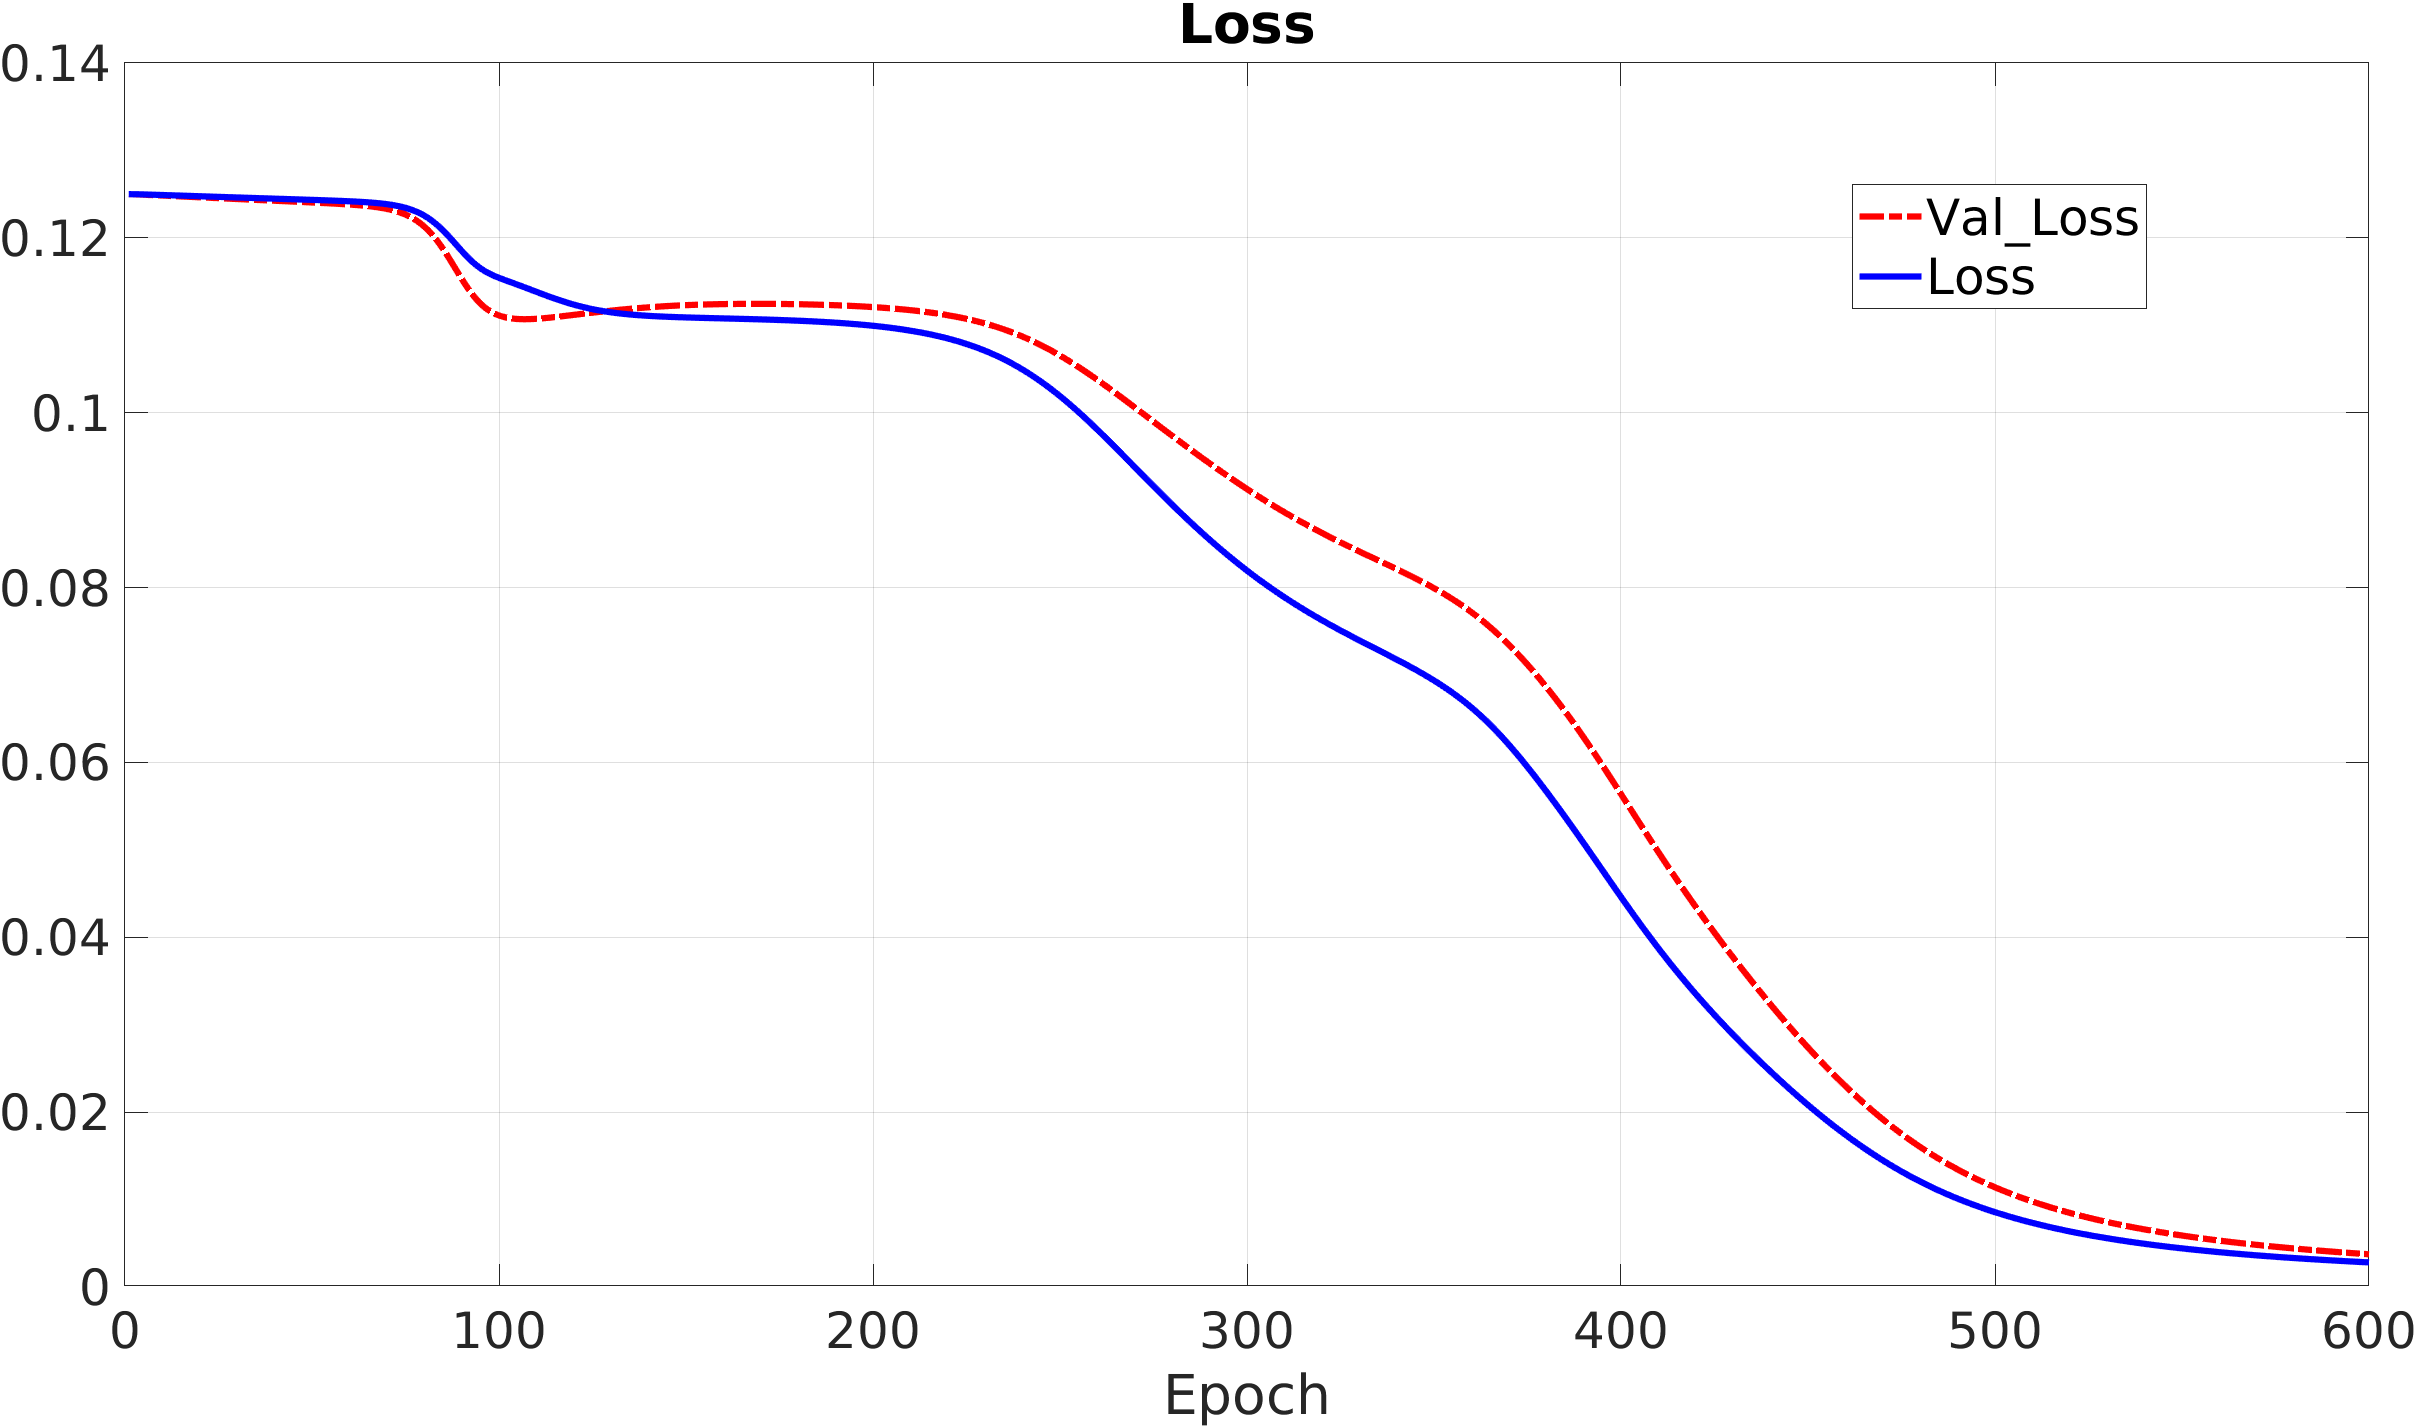
\includegraphics[width=\linewidth]{img/Monk2_loss.png}
        %\subcaption{MSE}
    \end{minipage}%
    \begin{minipage}[t]{0.5\linewidth}
        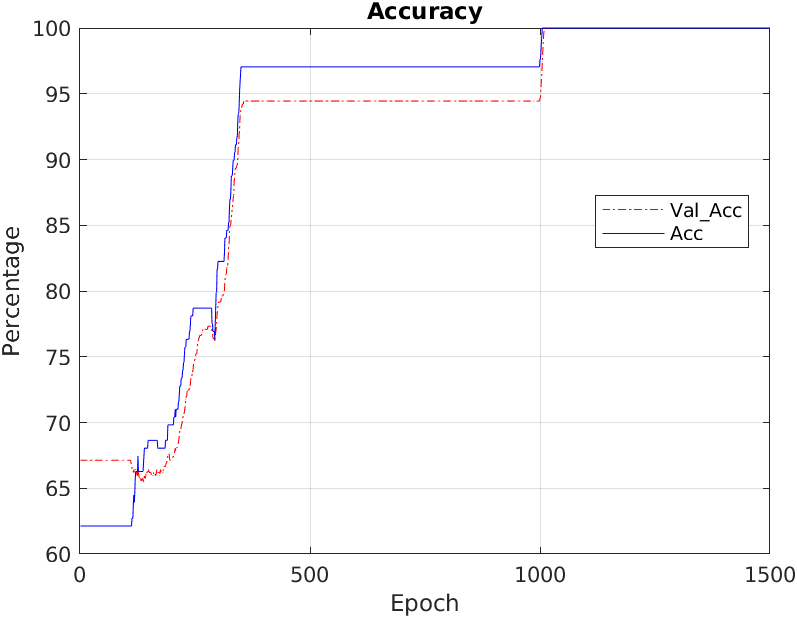
\includegraphics[width=\linewidth]{img/Monk2_accuracy.png}
        %\subcaption{Accuracy}
    \end{minipage}
    \caption{MSE and accuracy for MONK’s 2.}
\end{figure}

\subsubsection{Monk 3}
\begin{figure}[H]
    \centering
    \begin{minipage}[t]{0.5\linewidth}
        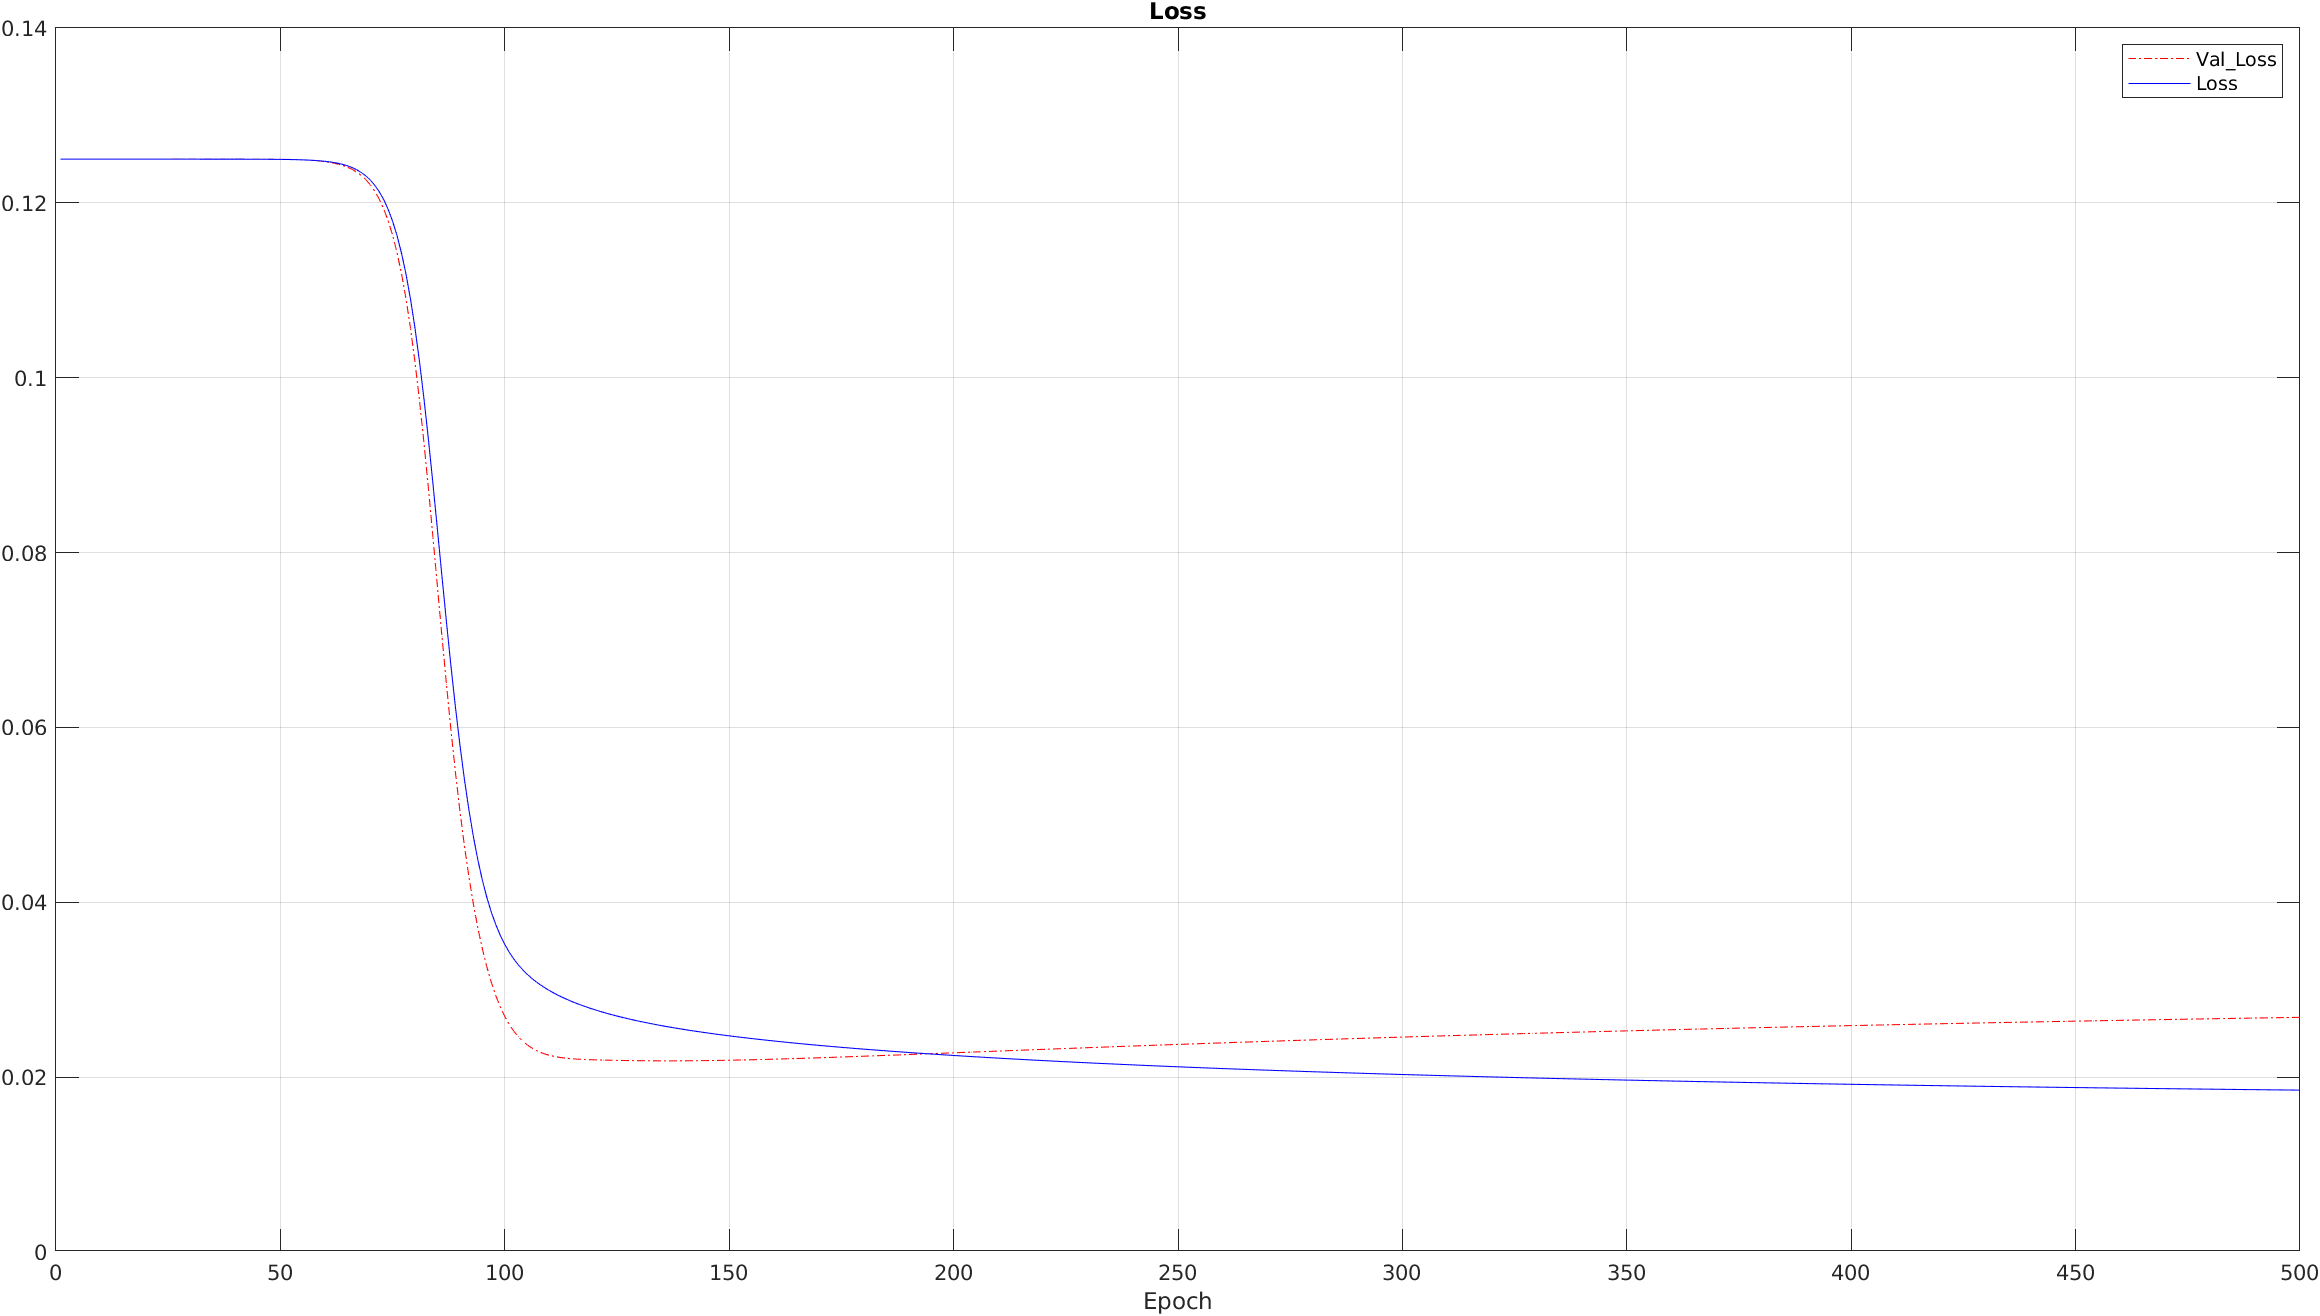
\includegraphics[width=\linewidth]{img/Monk3_loss_noReg.png}
        %\subcaption{MSE}
    \end{minipage}%
    \begin{minipage}[t]{0.5\linewidth}
        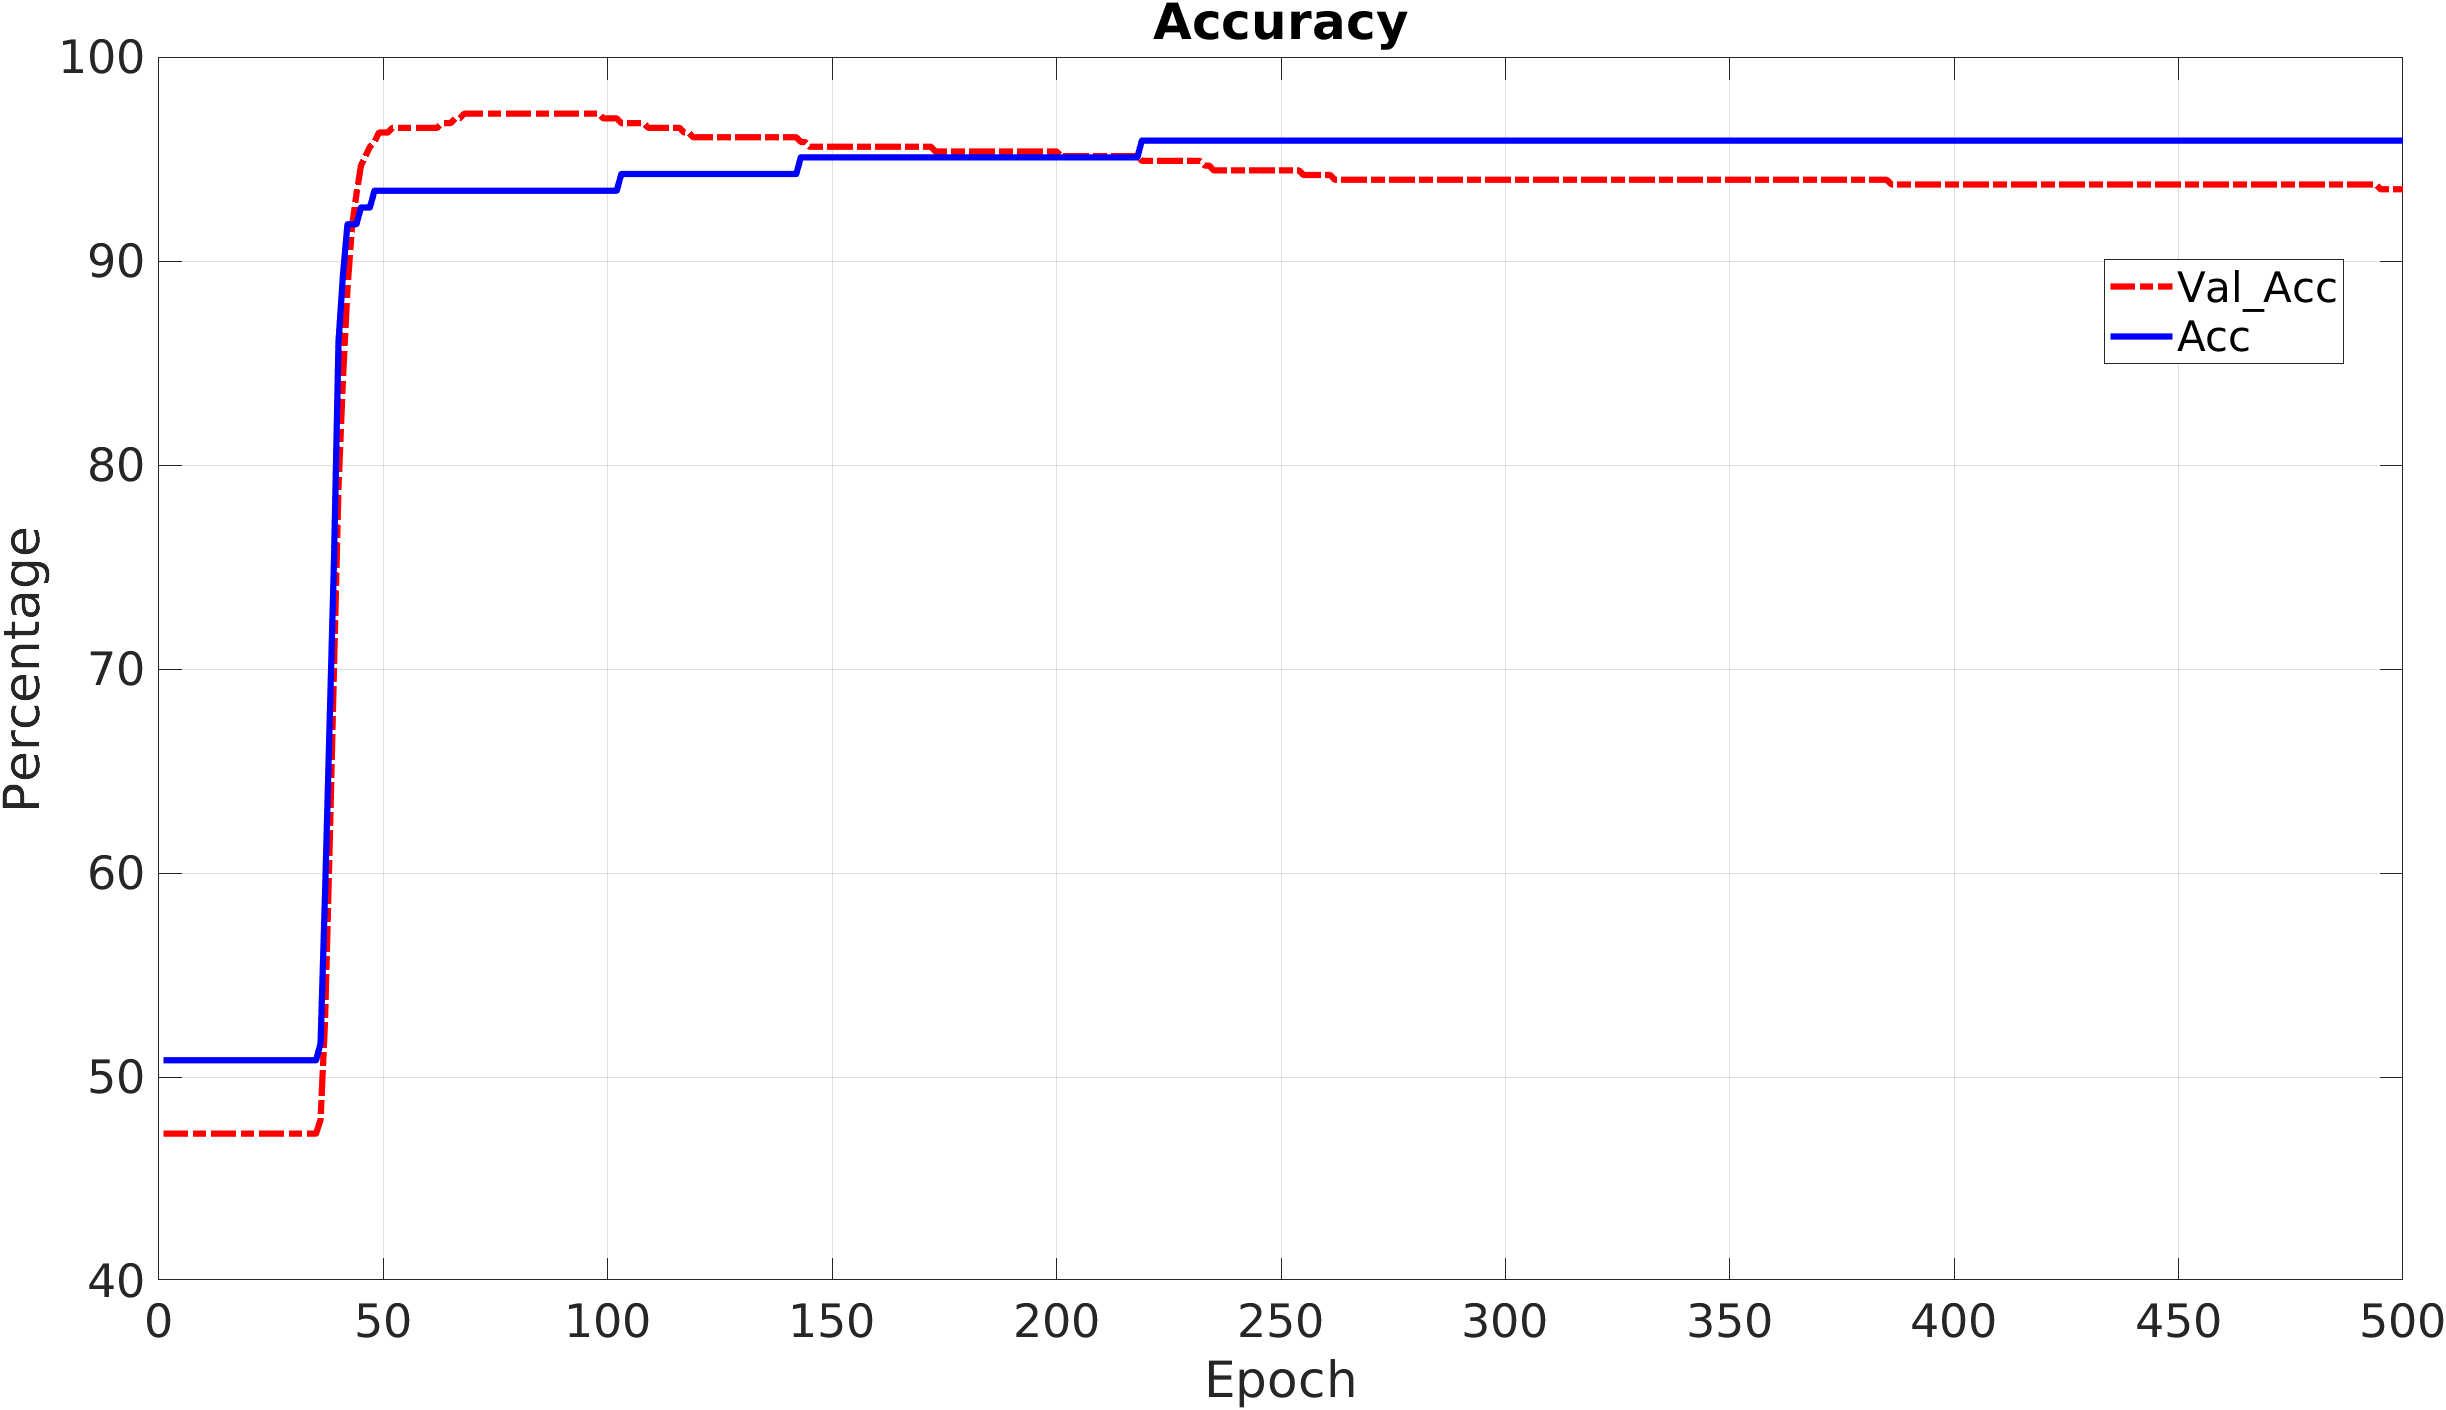
\includegraphics[width=\linewidth]{img/Monk3_accuracy_noReg.png}
        %\subcaption{Accuracy}
    \end{minipage}
    \caption{MSE and accuracy for MONK’s 3 not regularized.}
\end{figure}

\begin{figure}[H]
    \centering
    \begin{minipage}[t]{0.5\linewidth}
        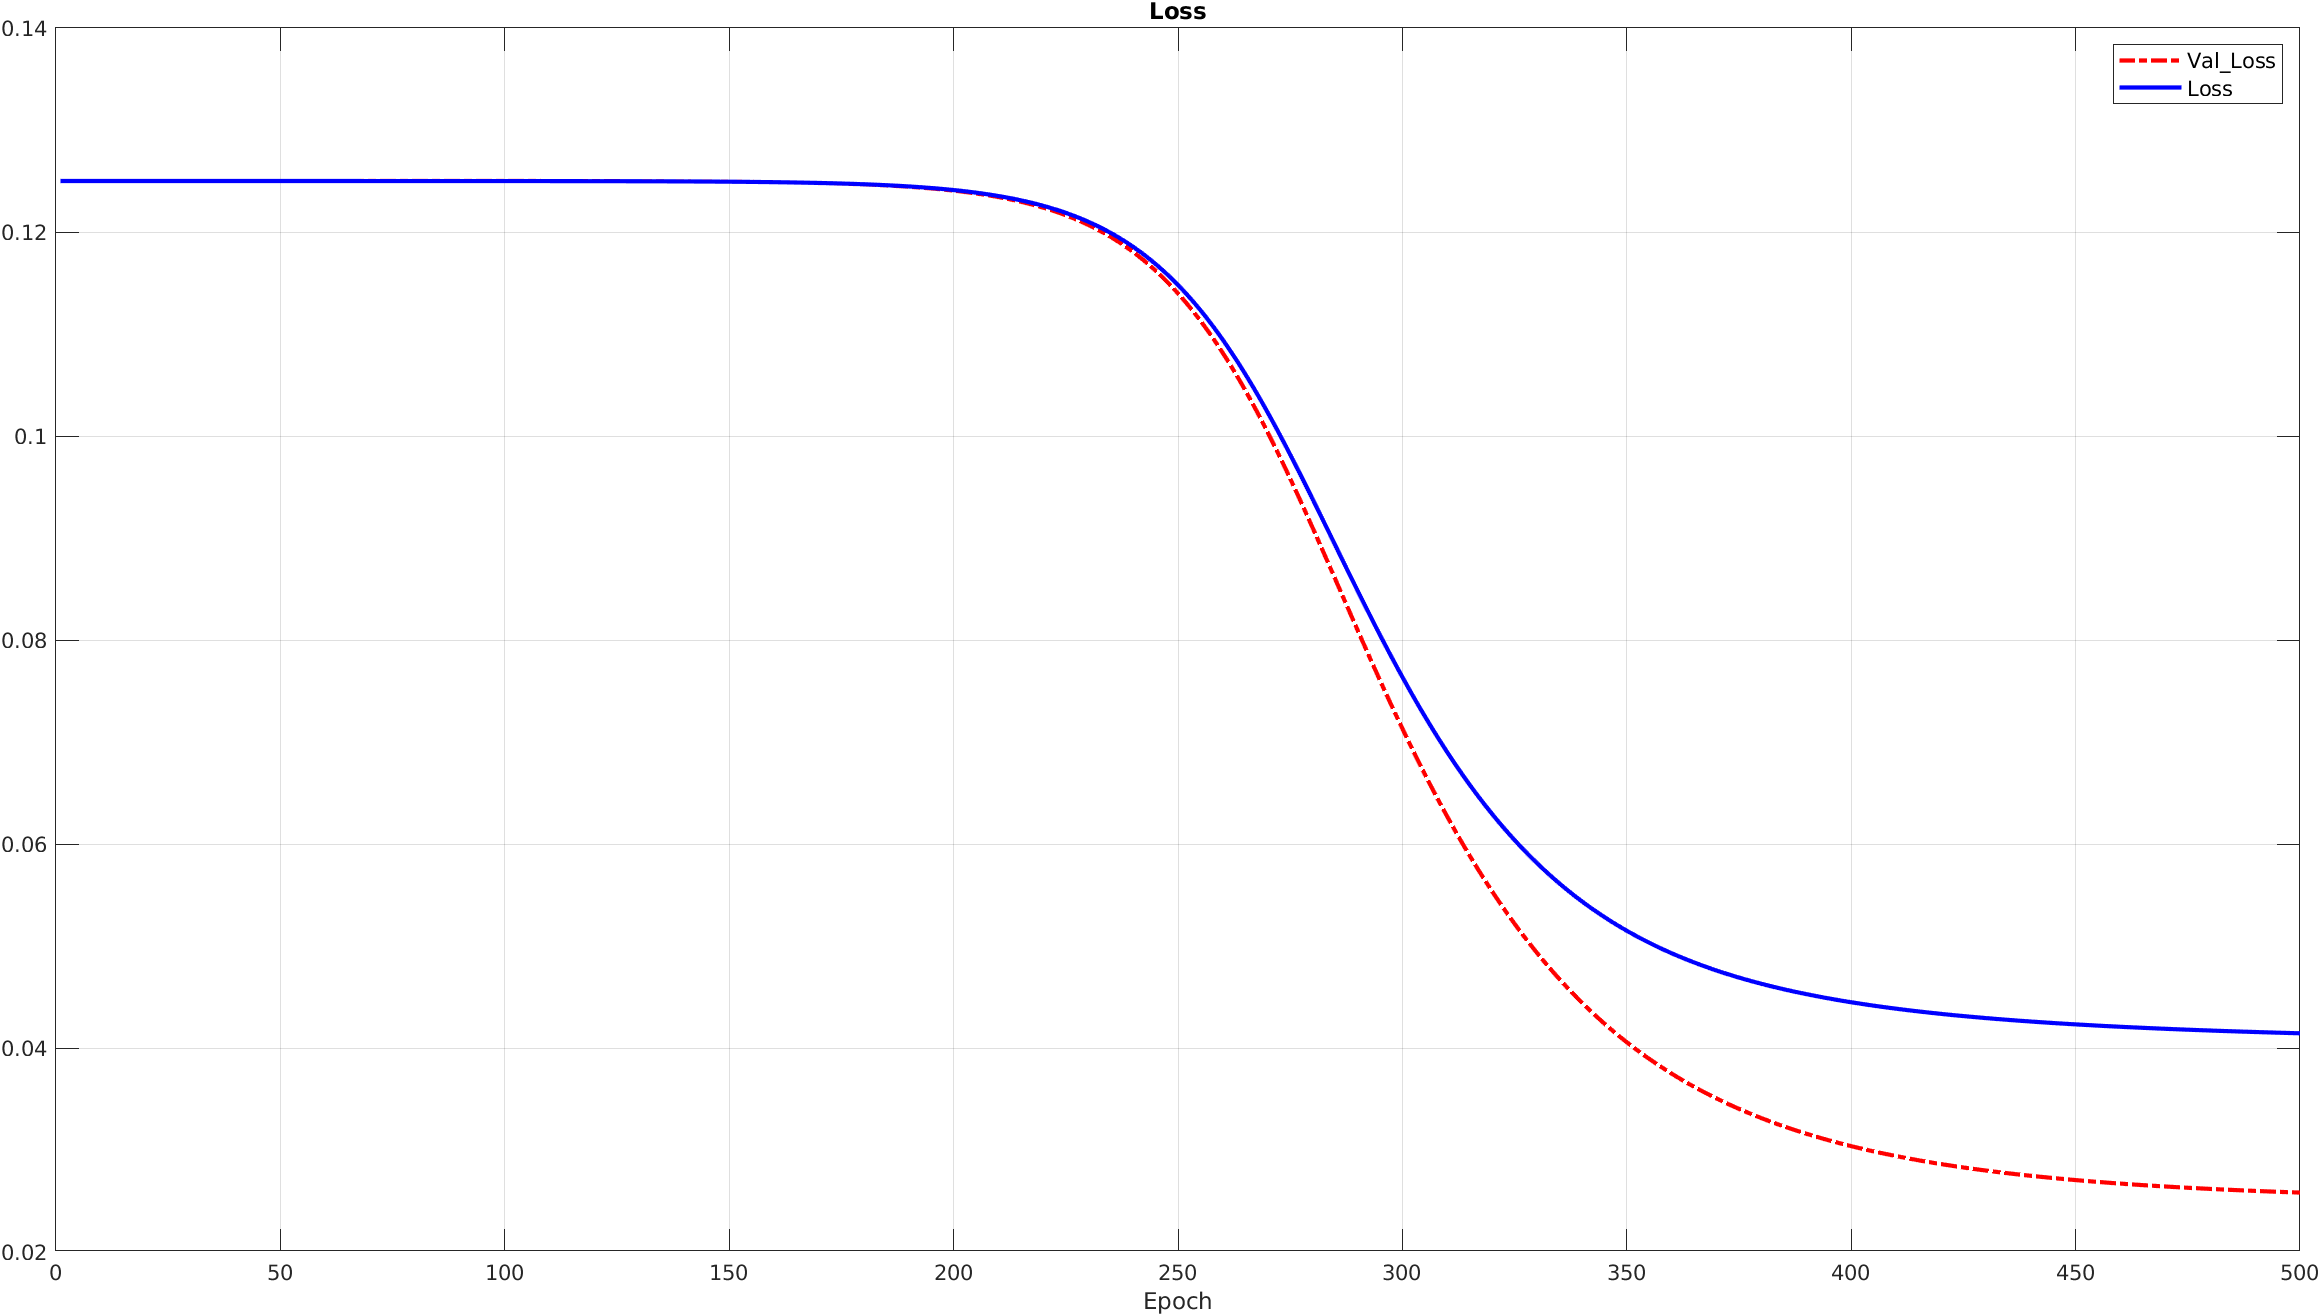
\includegraphics[width=\linewidth]{img/Monk3_loss_Reg.png}
        %\subcaption{MSE}
    \end{minipage}%
    \begin{minipage}[t]{0.5\linewidth}
        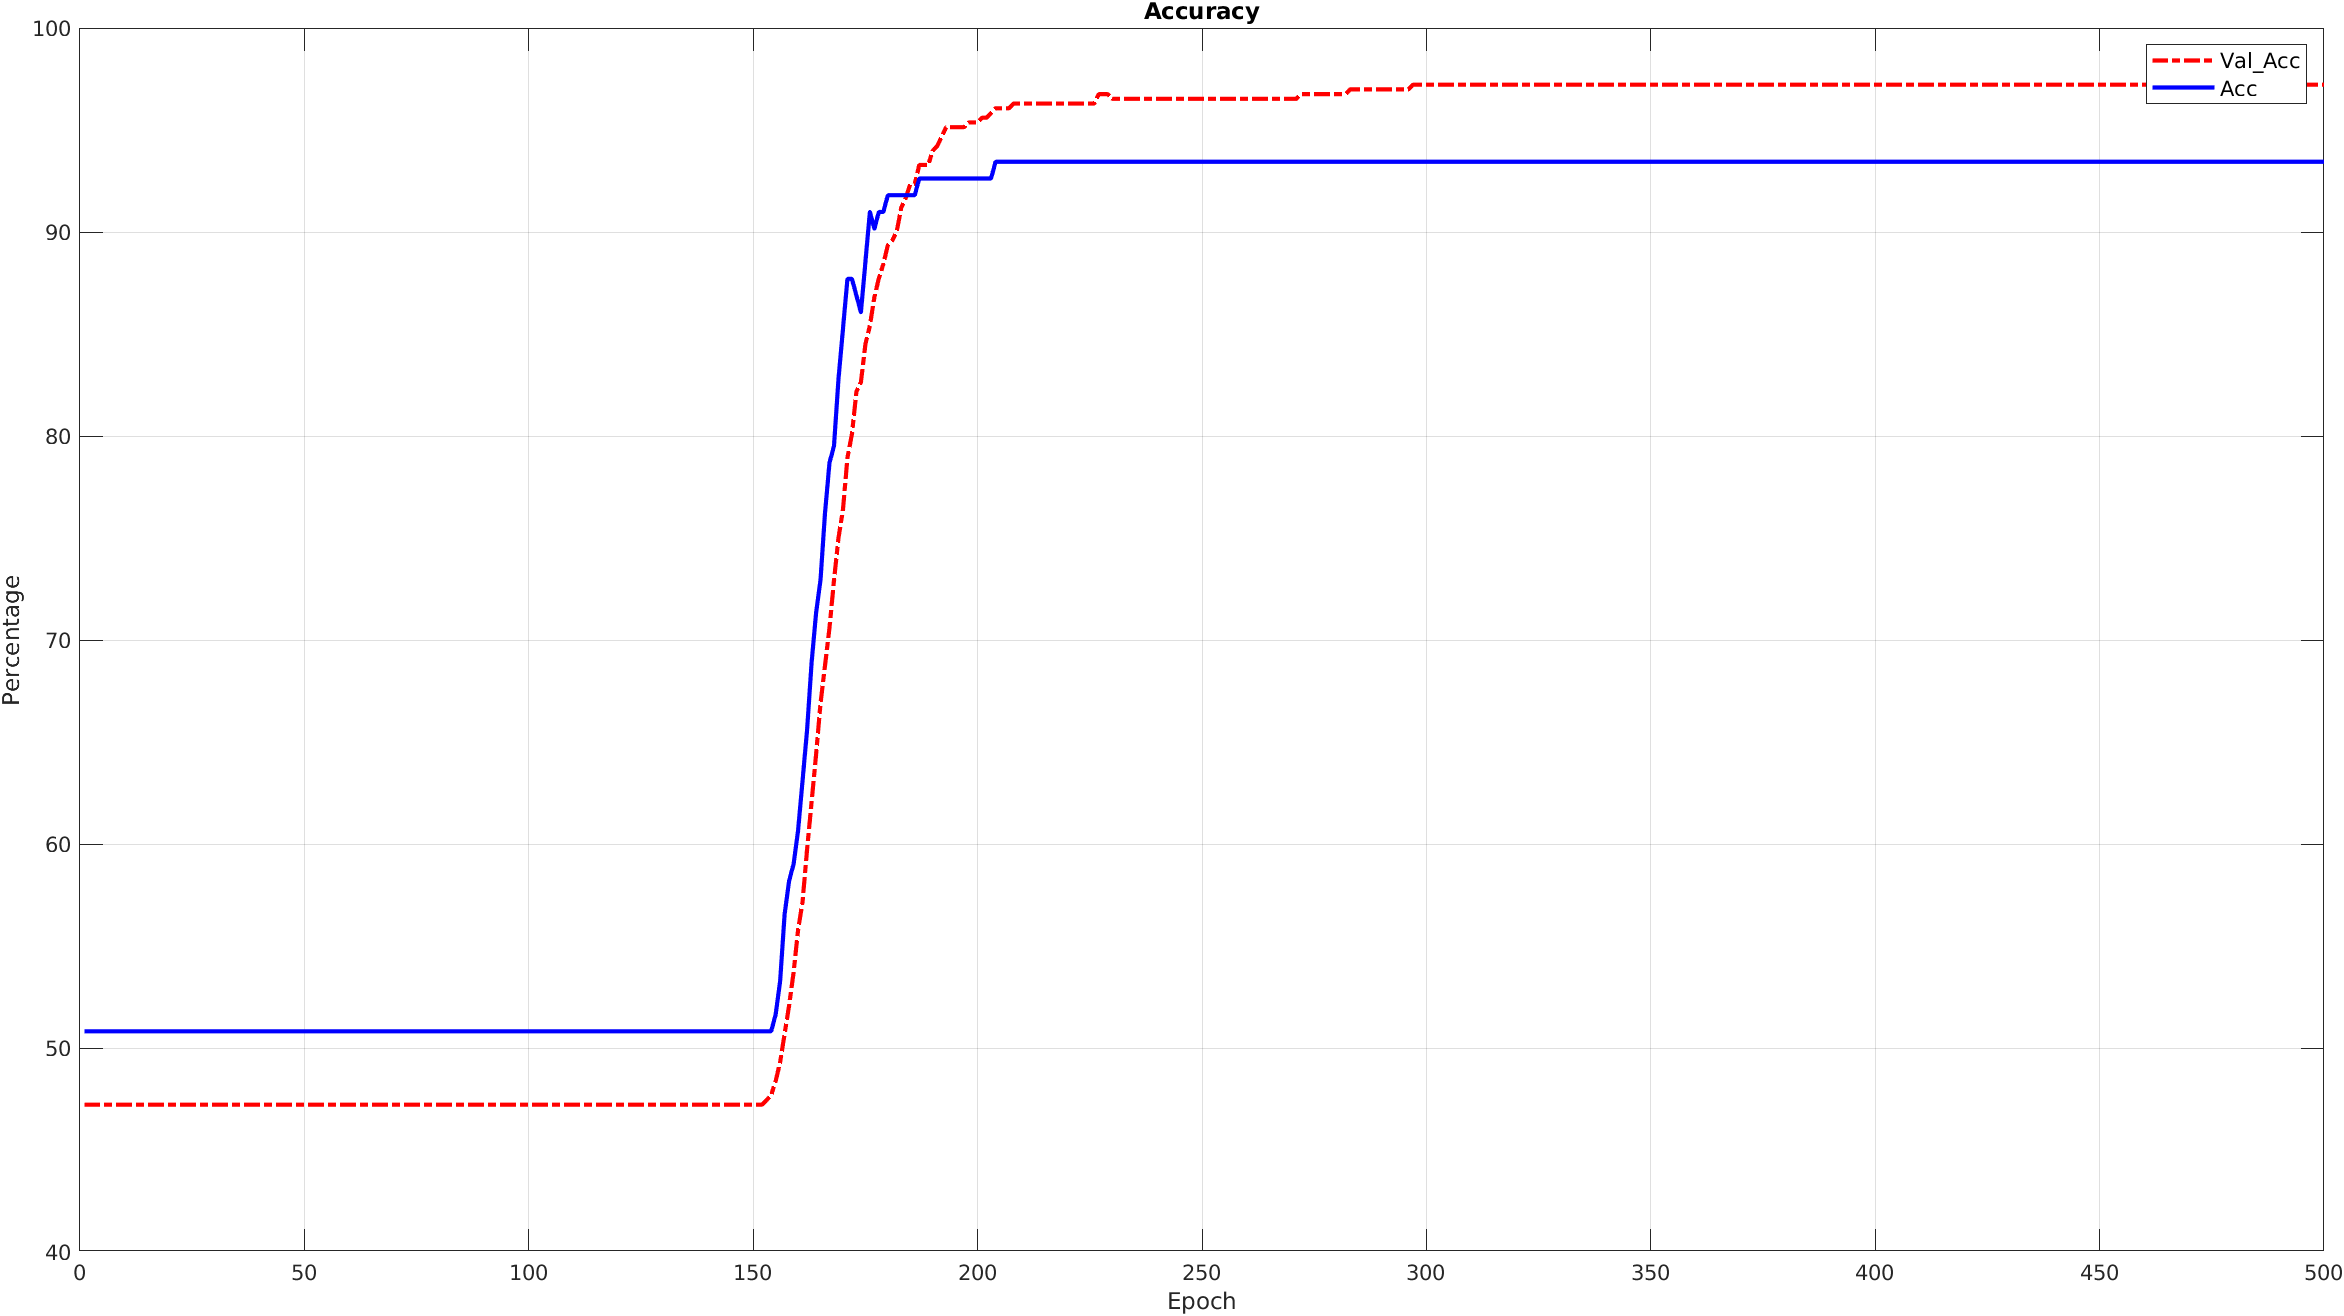
\includegraphics[width=\linewidth]{img/Monk3_accuracy_Reg.png}
        %\subcaption{Accuracy}
    \end{minipage}
    \caption{MSE and accuracy for MONK’s 3 regularized.}
\end{figure}



\subsection{Cup results}


\subsubsection{Validation schema}
\texttt{Details of the Validation schema (model selection and evaluation schema): Splitting  TR/VL/(internal)TS (data for each set and/or the K values of the k-fold CV)  [*]}
\subsubsection{Screening phase}
\texttt{Type of preliminary trials pursued (often summarized by text)}
\subsubsection{Explored hyper-parameters}
\texttt{Schema and  range of explored hyper-parameters (values used for the grid search, possibly a table) [*]}
\subsubsection{Grid search result}
\texttt{Grid search: TABLES of results TR/VL/(TS)i with  MEE [*]. At least the most performant cases. Tables/Plots can be used also to show some relevant trends for specific hyper-parameters changes (if you think it is significant) }
\subsubsection{Computing time}
\texttt{Provide an estimation of the (training) computing time (and of your HW resources)}
\subsubsection{Comparisons}
\texttt{Repeat and compare if you are comparing different models/algorithms/approaches (or different variants of the approach that you think are significant). }
\subsubsection{Chosen model}
\texttt{Define how you selected the FINAL model used on the blind test set [*]. Which is it among the candidates and why? Also write the  hyper-param. of the final model [*].}
\subsubsection{Report}
\texttt{Report for the FINAL model used on the blind test set the TABLE with MEE for TR (training), VL (validation) and TS (internal TS)i  in the original scale [*][*]. Note again  that you must have an internal  test evaluation (see the note IV above)}
\subsubsection{Plots}
\texttt{Plot the learning curve TR/(VL)i/TS for the FINAL model [*] (the final model is unique) }
\begin{figure}[H]
    \centering
    \begin{minipage}[t]{0.5\linewidth}
        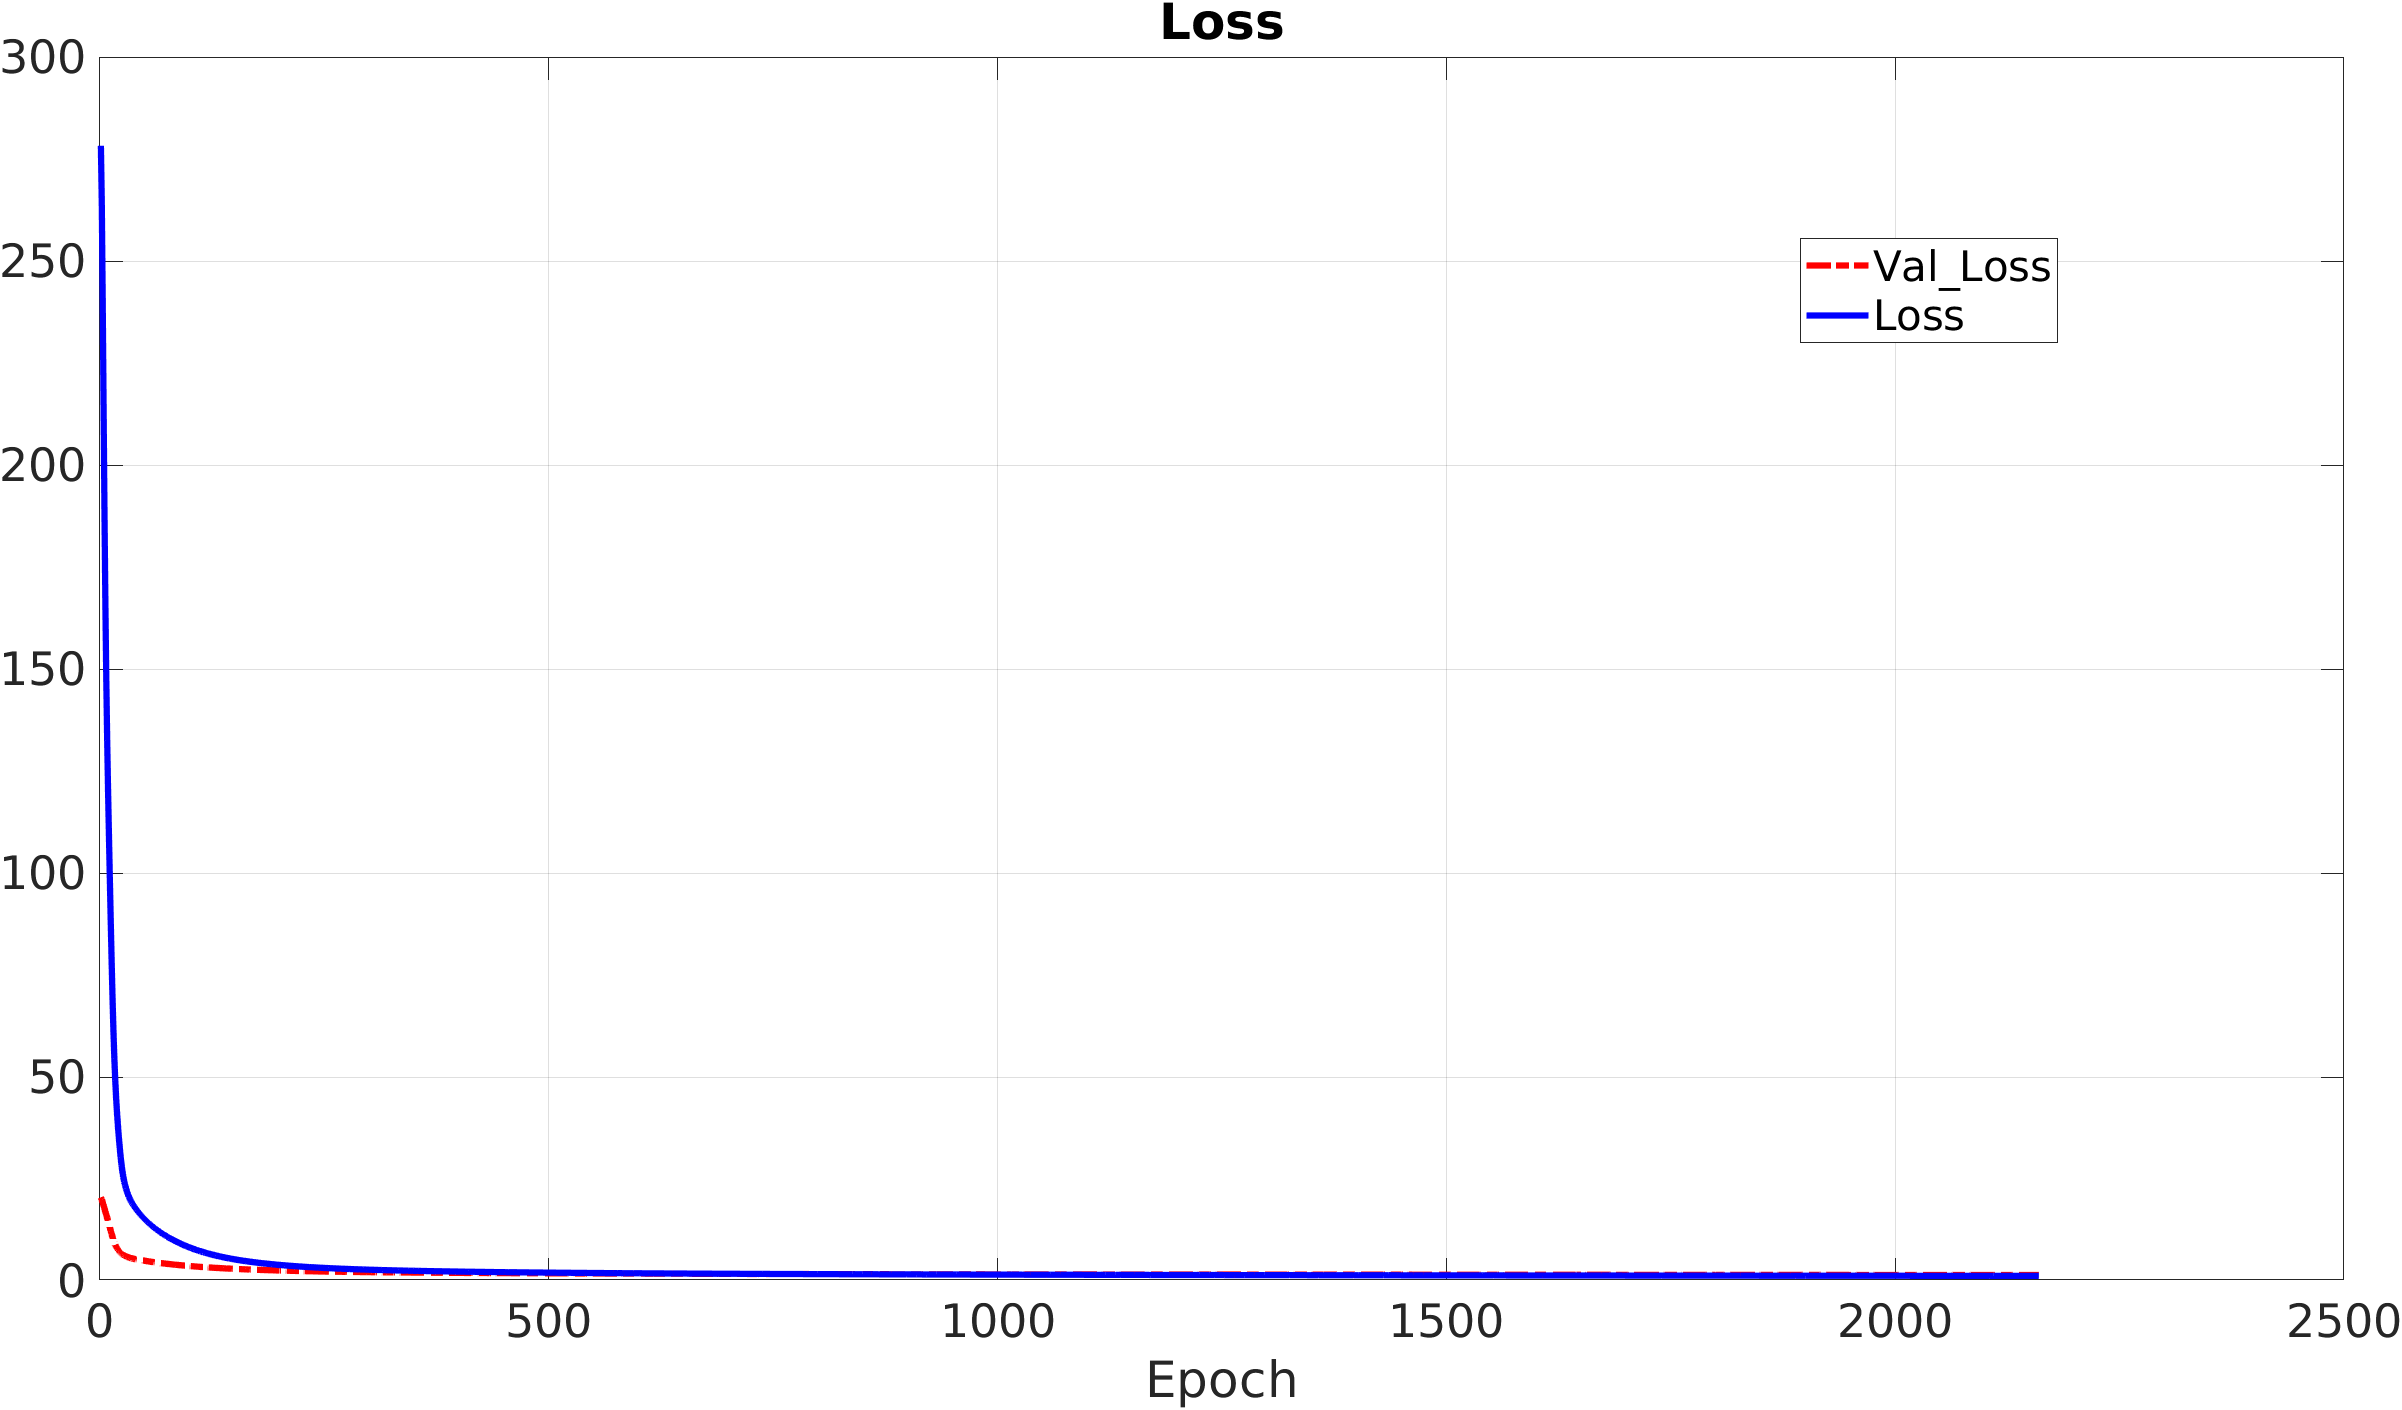
\includegraphics[width=\linewidth]{img/Cup_loss_noReg_noZoom.png}
        %\subcaption{MSE}
    \end{minipage}%
    \begin{minipage}[t]{0.5\linewidth}
        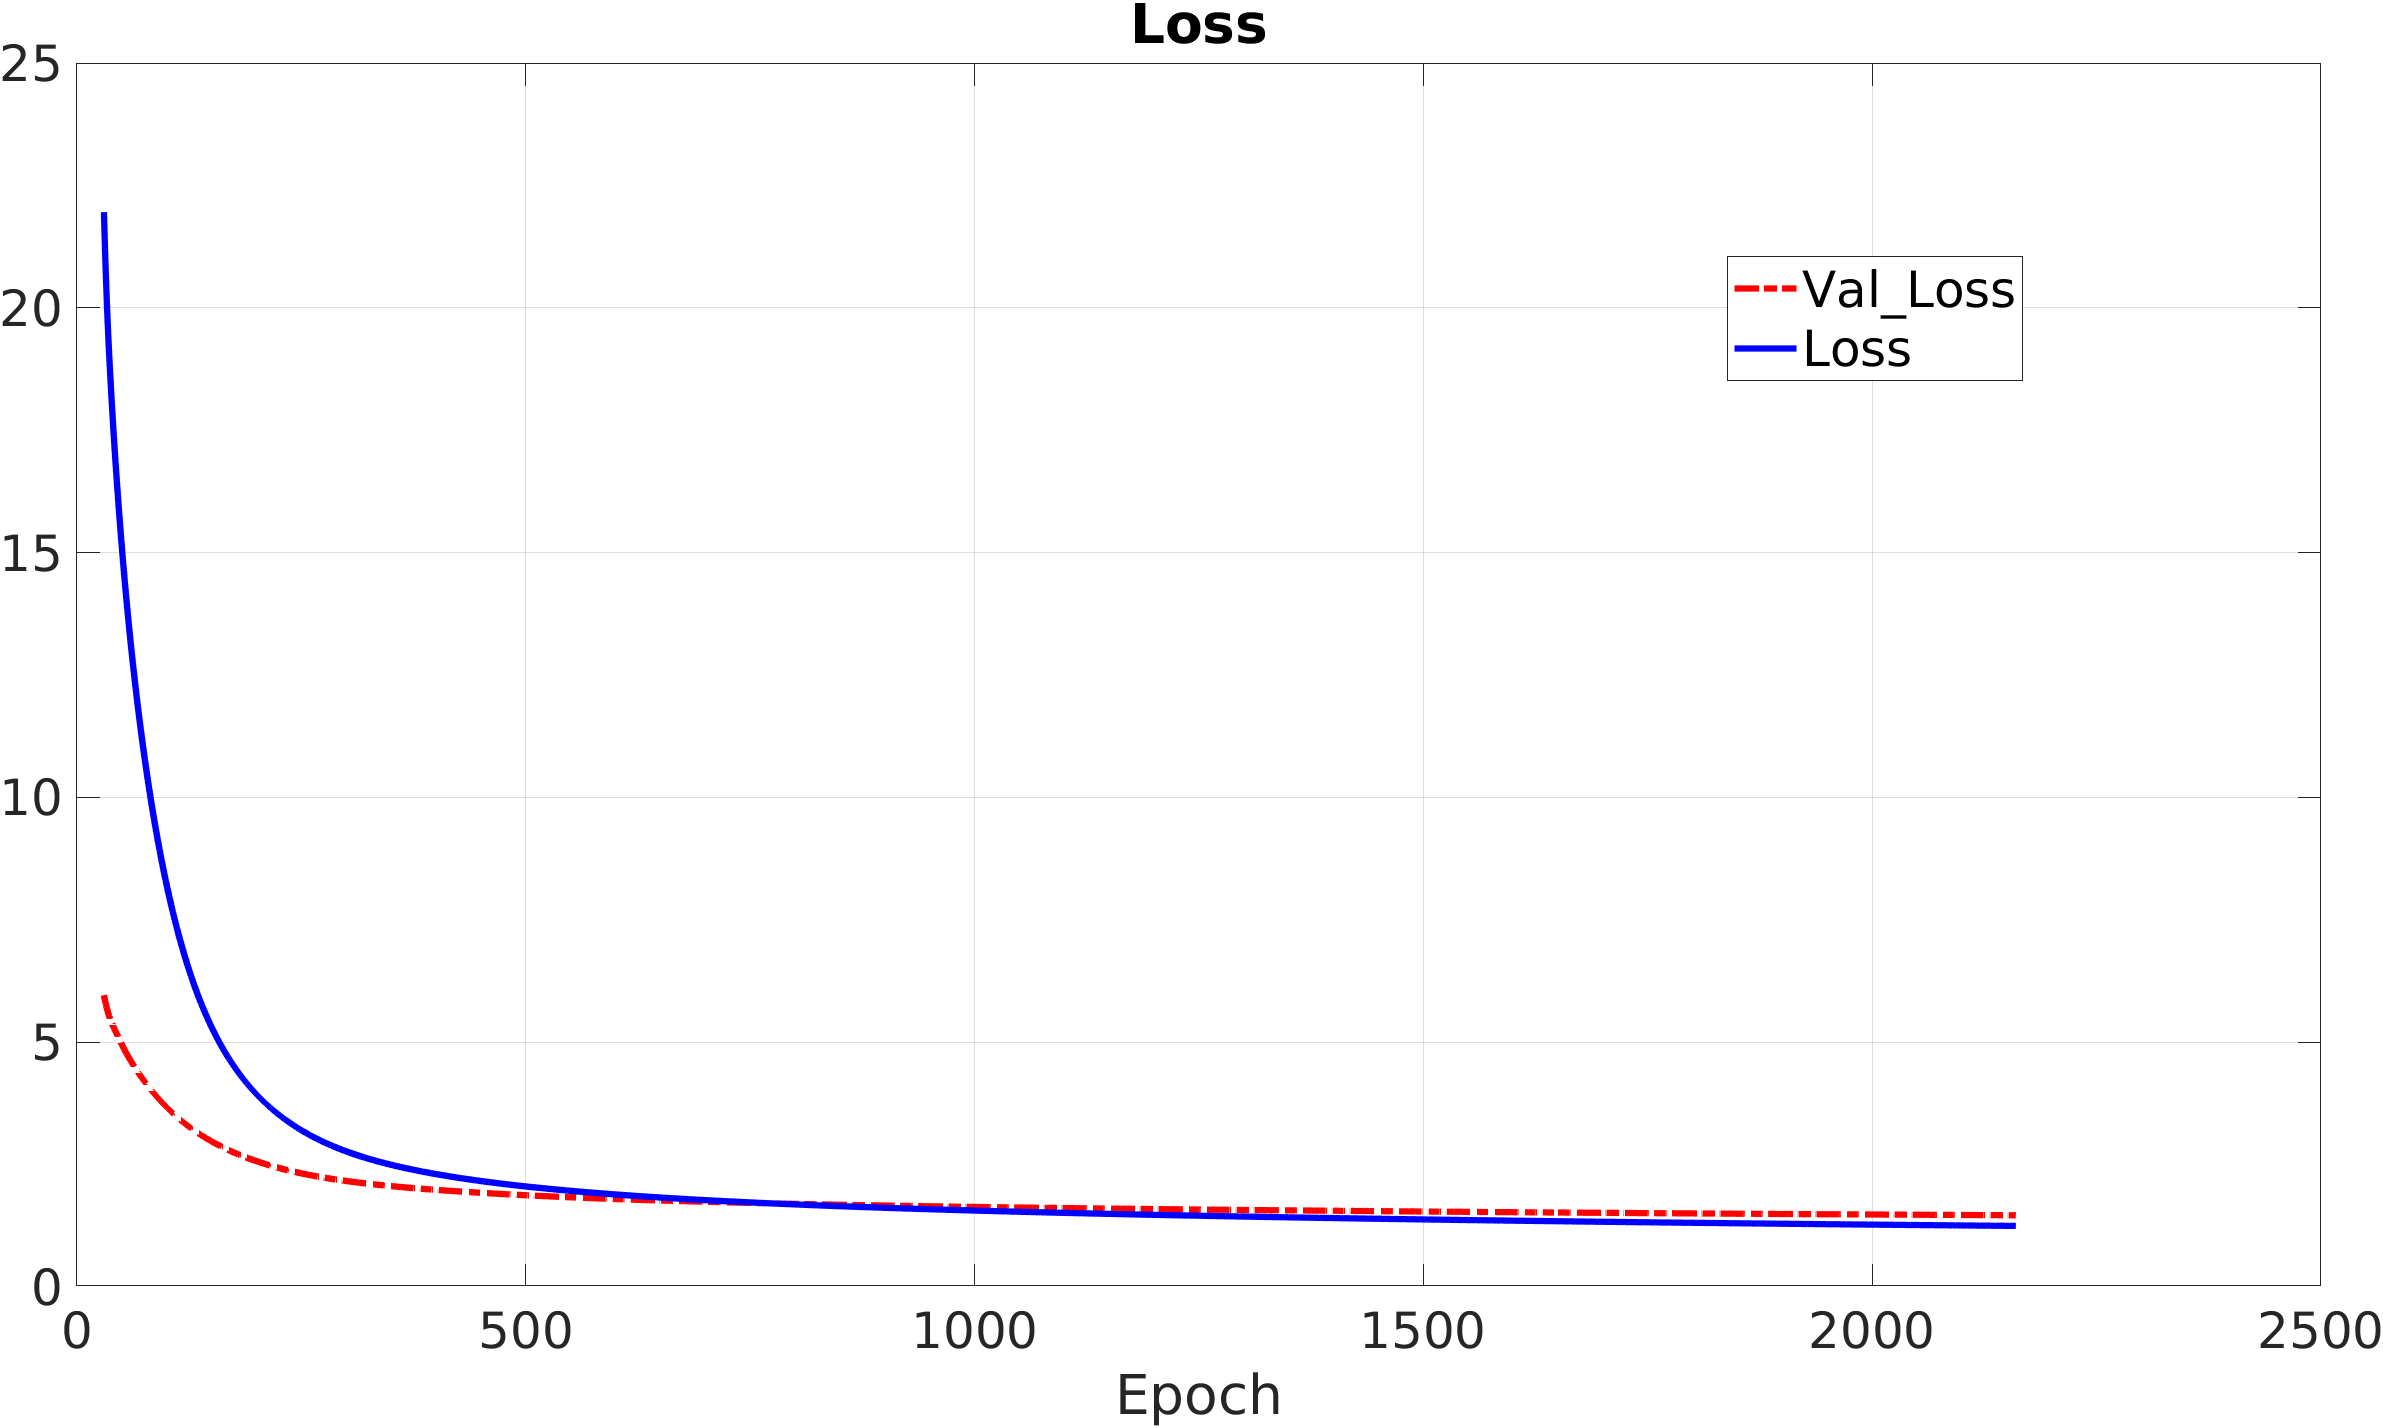
\includegraphics[width=\linewidth]{img/Cup_loss_noReg_zoom.png}
        %\subcaption{Accuracy}
    \end{minipage}
    \caption{MEE and zoomed MEE for ML cup not regularized.}
\end{figure}

\begin{figure}[H]
    \centering
    \begin{minipage}[t]{0.5\linewidth}
        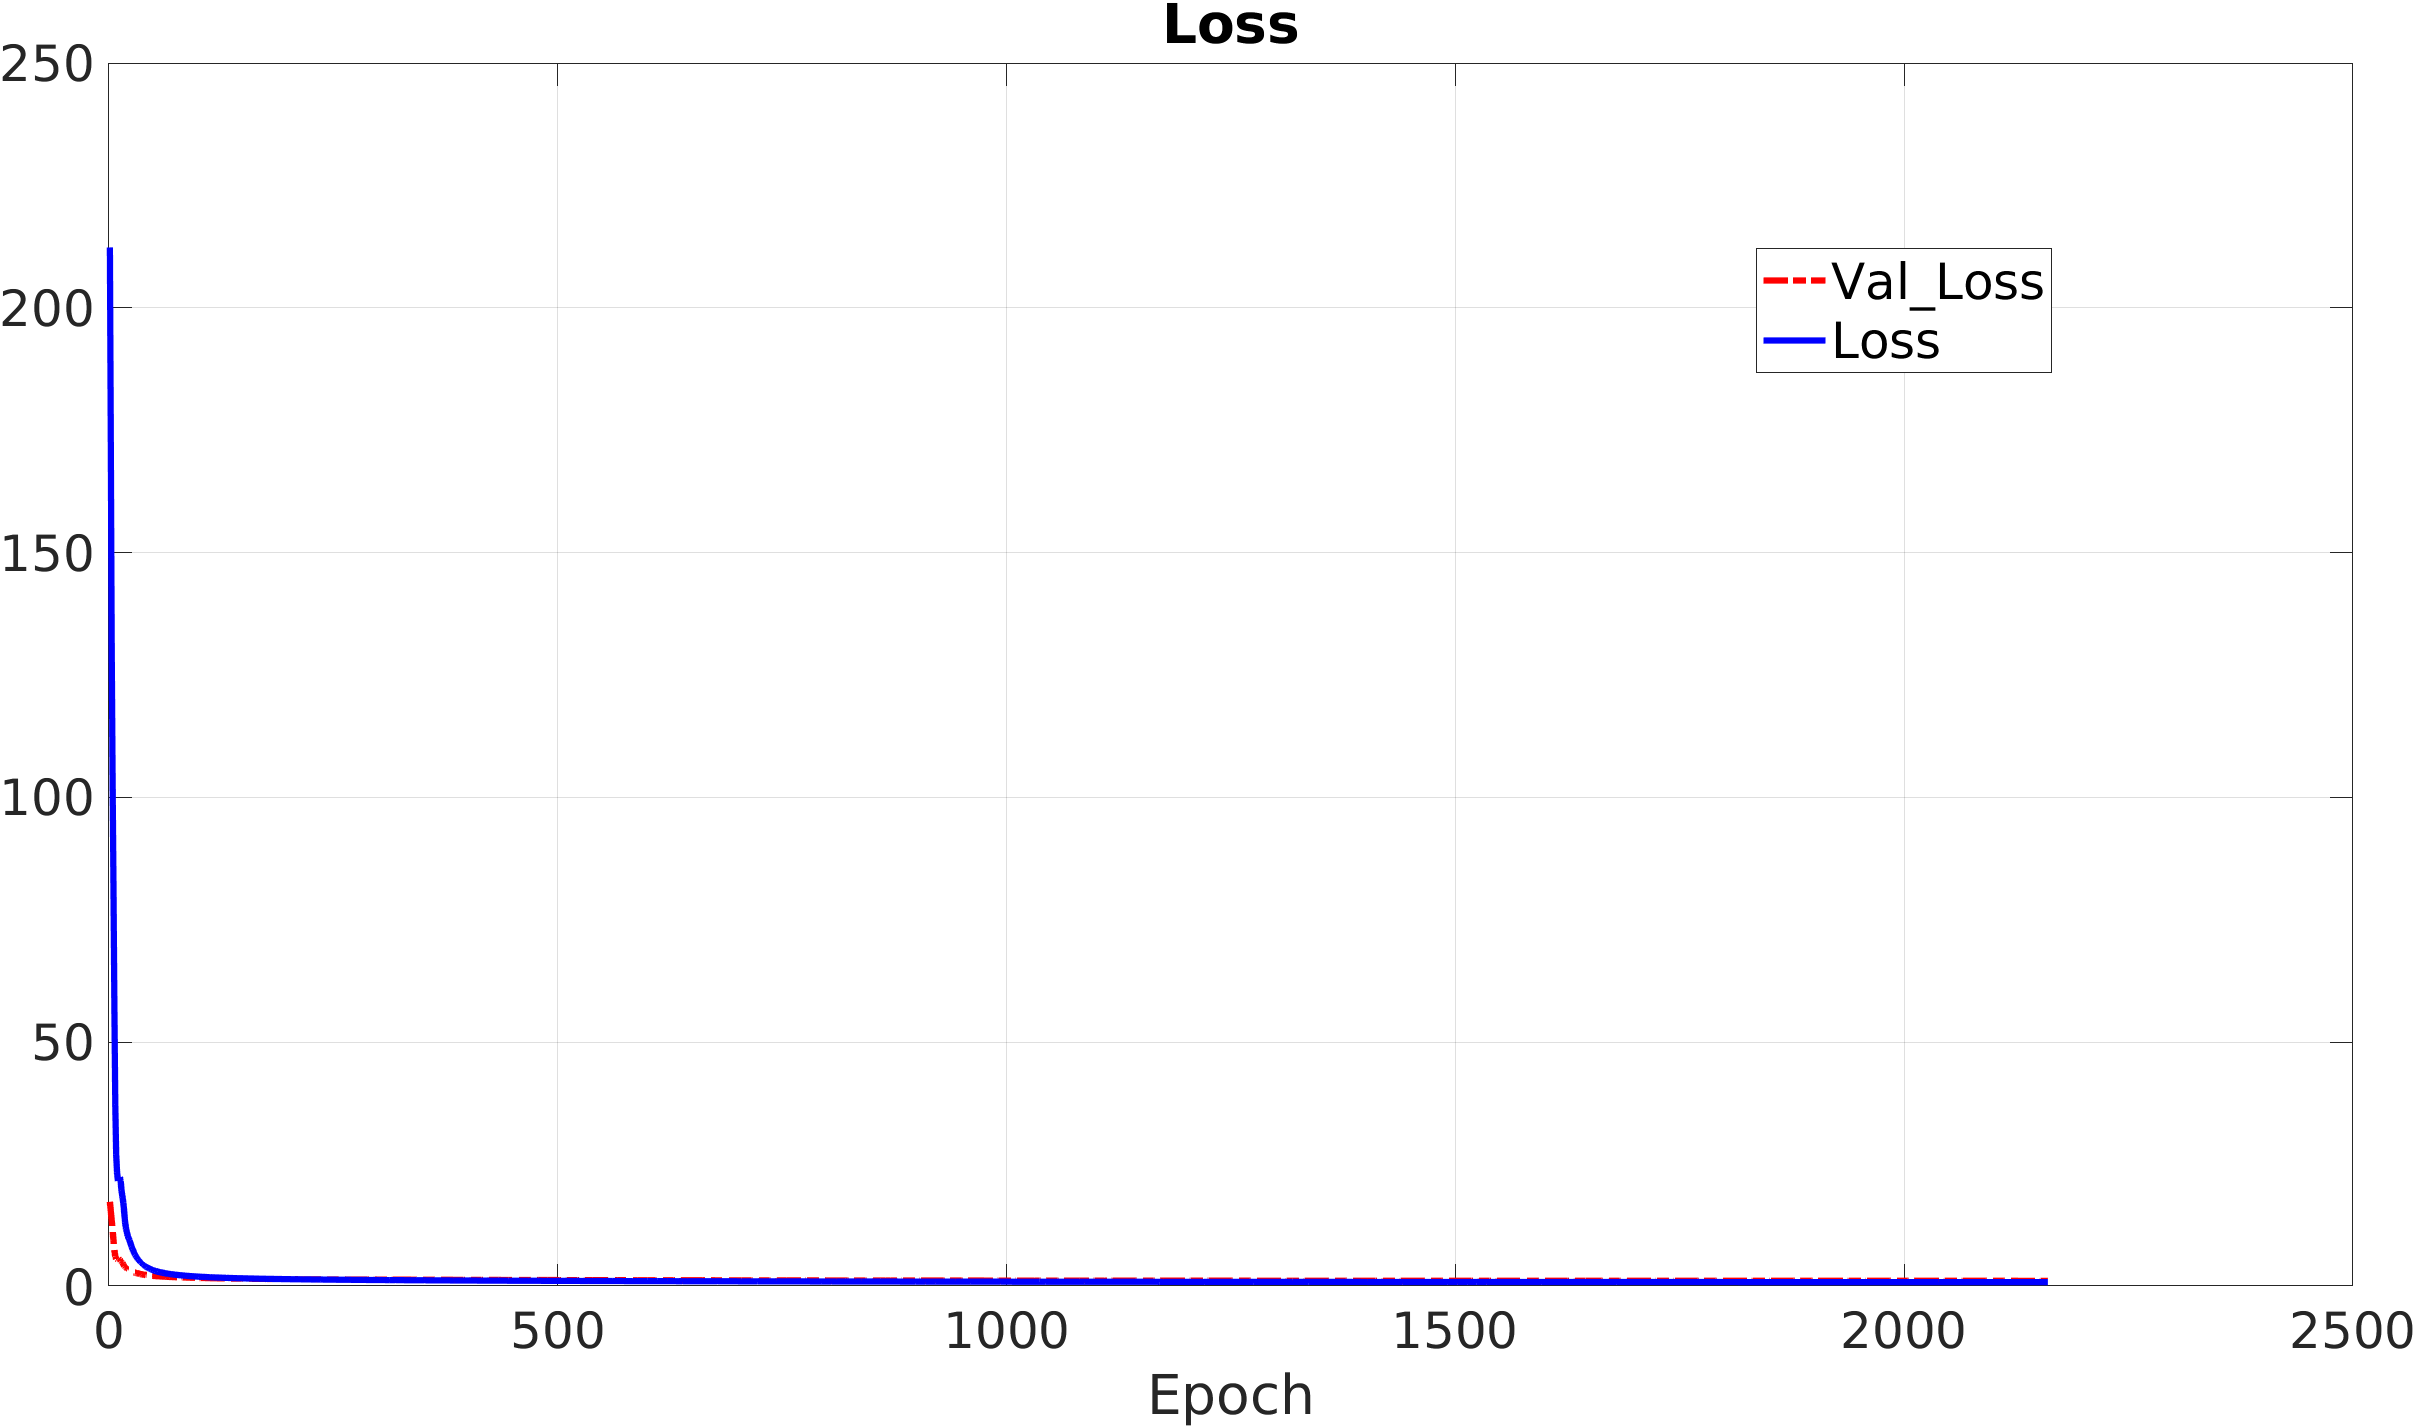
\includegraphics[width=\linewidth]{img/Cup_loss_Reg_noZoom.png}
        %\subcaption{MSE}
    \end{minipage}%
    \begin{minipage}[t]{0.5\linewidth}
        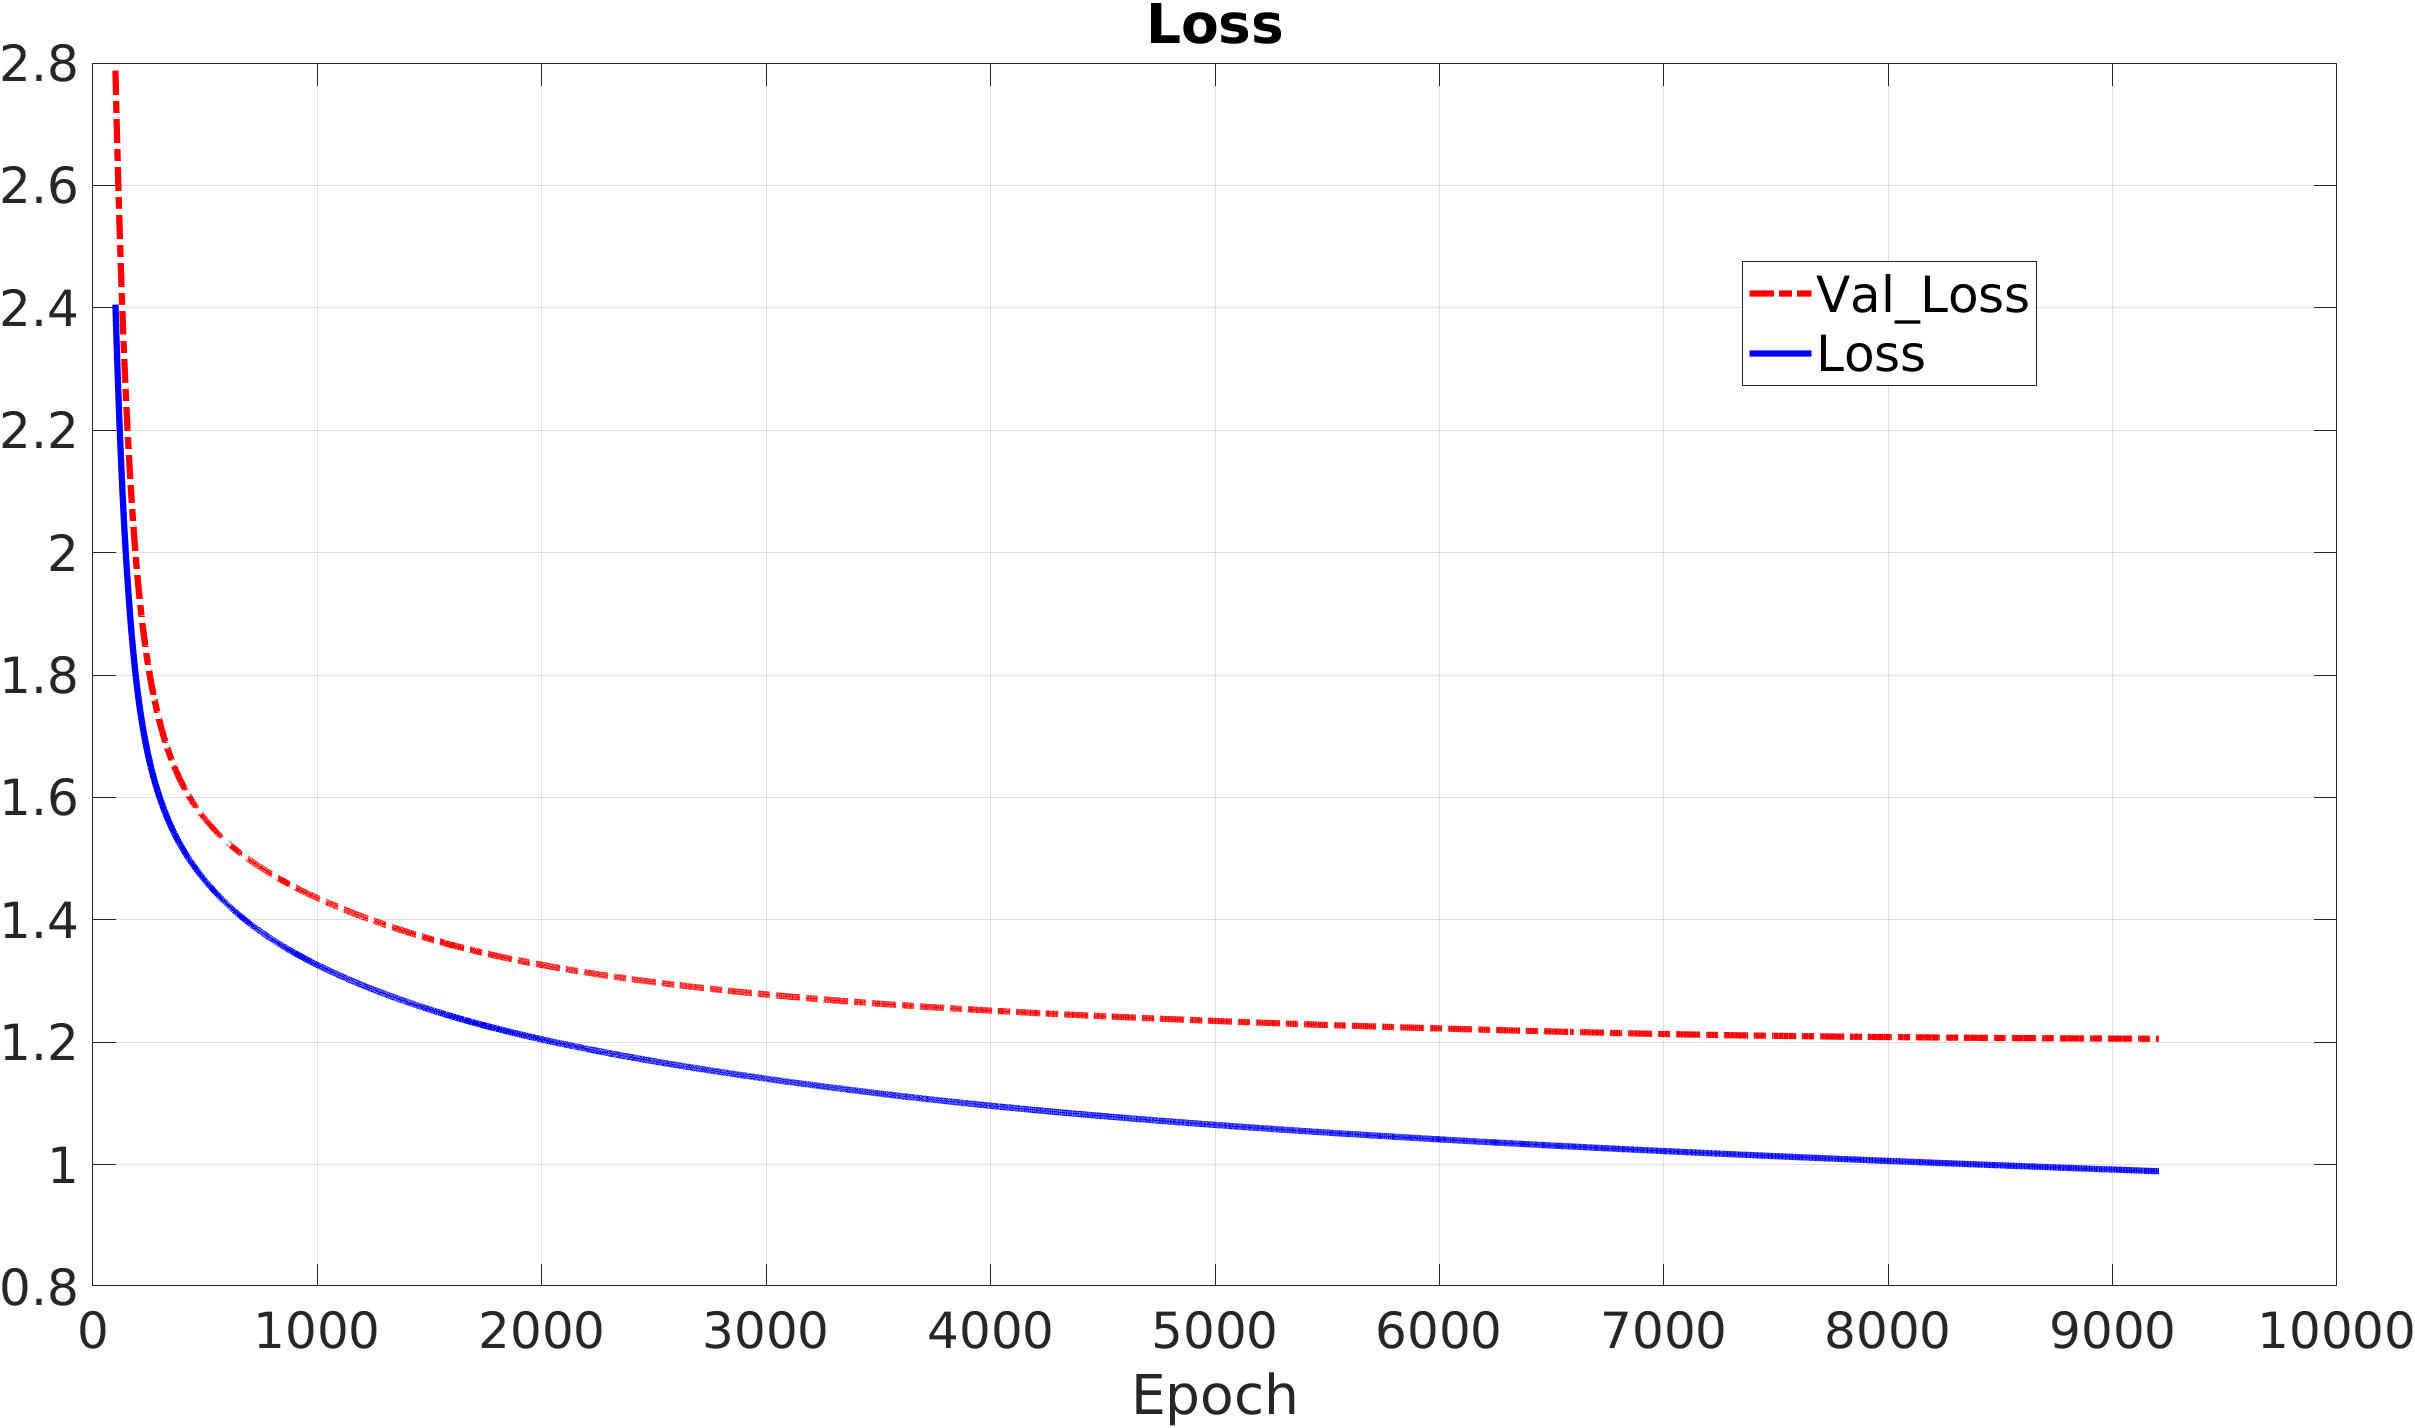
\includegraphics[width=\linewidth]{img/Cup_loss_Reg_Zoom.png}
        %\subcaption{Accuracy}
    \end{minipage}
    \caption{MEE and zoomed MEE for ML cup regularized.}
\end{figure}



